\documentclass[a4paper,14pt]{extarticle}

% Шрифты, кодировки, символьные таблицы, переносы
\usepackage{cmap}
\usepackage[T2A]{fontenc}
\usepackage[utf8x]{inputenc}
\usepackage[english, russian]{babel}

% Пакеты американского математического сообщества
\usepackage{amssymb,amsfonts,amsmath,amsthm}  
% Сокращения
\usepackage{cancel}

\theoremstyle{definition}
\newtheorem{definition}{Определение}

% Красная строка
\usepackage{indentfirst}

% Ссылки в pdf
\usepackage[unicode, colorlinks, urlcolor=magenta, linkcolor=black]{hyperref}

% Таблицы
\usepackage{makecell,multirow} 

% Графика
\usepackage{graphicx}
\usepackage[usenames,dvipsnames]{color} 
\usepackage{float}
% \usepackage{subcaption}

% Геометрия страницы
\usepackage{geometry}
\geometry{left=2cm,right=2cm,top=2.5cm,bottom=2.5cm,bindingoffset=0cm,headheight=18pt}

% Колонтитулы
\usepackage{fancyhdr} 
% применим колонтитул к стилю страницы
\pagestyle{fancy} 
%очистим "шапку" страницы
\fancyhead{} 
%слева сверху на четных и справа на нечетных
\fancyhead[R]{Лекции В.И. Некоркина 2018-2019} 
% \fancyhead[R]{Сарафанов Ф.Г., Понур К.А. и др.} 
%справа сверху на четных и слева на нечетных
\fancyhead[L]{Теория колебаний} 
%очистим "подвал" страницы
\fancyfoot{} 
% номер страницы в нижнем колинтуле в центре
\fancyfoot[C]{\thepage} 

% Межстрочный отступ
\usepackage{setspace}
\linespread{1.15} % капельку увеличенный
\frenchspacing % <<французские>> пробелы

% Нумерация
\renewcommand{\labelenumii}{\theenumii)}
% В заголовках появляется точка, но при ссылке на них ее нет
\usepackage{misccorr}

% Содержание
\usepackage{tocloft}
\usepackage{secdot}
\sectiondot{subsection}

% Физика
\usepackage{physics}

% Новые команды
\newcommand{\Mean}[1]{\langle#1\rangle}
\newcommand{\Defi}{\underset{def}{=}}
\newcommand{\Inte}{\int\limits_{-\infty}^{\infty}} 

\addto\captionsrussian{%
	\renewcommand{\contentsname}{Оглавление}
	\renewcommand{\partname}{Раздел}%
}
\def\thepart{\arabic{part}}
\usepackage{tocloft}
\renewcommand{\cftpartleader}{\cftdotfill{\cftdotsep}} % for parts
% \renewcommand{\cftchapleader}{\cftdotfill{\cftdotsep}} % for chapters
\renewcommand{\cftsecleader}{\cftdotfill{\cftdotsep}} % for chapters
% \newlength\mylen
\renewcommand\thepart{\arabic{part}.}
% \renewcommand\cftpartpresnum{Лекция~}
% \renewcommand\cftsecpresnum{Лекция~}

% \setlength{\cftsecnumwidth}{6em}
% \renewcommand{\cftsecpresnum}{Лекция\ }
\renewcommand{\cftsecaftersnum}{.}

% \renewcommand{\cftsecaftersnumb}{\newline}
\renewcommand{\cftsecdotsep}{\cftdotsep}
\renewcommand{\kappa}{\varkappa}
\renewcommand{\phi}{\varphi}
\renewcommand{\epsilon}{\varepsilon}

% #1: math symbol
% #2: legend
\def\alegend#1#2{\overset{\underset{\scriptstyle\downarrow}{\scriptstyle\text{#2}}}{#1}}
\def\blegend#1#2{\underset{\underset{\scriptstyle\text{#2}}{\scriptstyle\uparrow}}{#1}}
\def\hp{\hat{p}}
\def\hx{\hat{x}}
\def\hH{\hat{H}}

\usepackage[explicit]{titlesec}
% \titleformat{\section}{\normalfont\Large\bfseries}{}{0em}{Лекция\ \thesection.\ #1}
\usepackage{epigraph}


\newcommand\praktika[1]{
\stepcounter{section}
\vspace{1.5em}
\noindent\textbf{\Large{Занятие \arabic{section}.\hspace{.2em} #1}}
% \newline 
\vspace{-0.5em}
\addcontentsline{toc}{section}{Занятие \arabic{section}.\hspace{.5em} #1}
}

% \usepackage{mathtools}
% \mathtoolsset{showonlyrefs=true}


% https://tex.stackexchange.com/questions/8720/overbrace-underbrace-but-with-an-arrow-instead

\usepackage{xparse}% http://ctan.org/pkg/xparse

\NewDocumentCommand{\overarrow}{O{=} O{\uparrow} m}{%
  \overset{\makebox[0pt]{\begin{tabular}{@{}c@{}}$#3$\\[0pt]\ensuremath{#2}\end{tabular}}}{#1}
}
\NewDocumentCommand{\underarrow}{O{=} O{\downarrow} m}{%
  \underset{\makebox[0pt]{\begin{tabular}{@{}c@{}}\ensuremath{#2}\\[0pt]$#3$\end{tabular}}}{#1}
}

\newcommand\undernoteqty[2]{
	%
	\underarrow[
		\qty(\underbrace{#1})
	][\uparrow]{\substack{#2}}
	%
}

\newcommand{\pvec}[1]{\vec{#1}\mkern2mu\vphantom{#1}}
% Нормальный вектор для штрихов
\newcommand{\phat}[1]{\hat{#1}\mkern2mu\vphantom{#1}}

\newcommand\undernote[2]{
	%
	\underarrow[
		#1
	][\uparrow]{\substack{#2}}
	%
}



% ##############################################################################
% ##############################################################################
\newcommand*\dotvec[1][1,1]{\crossproducttemp#1\relax}
\def\crossproducttemp#1,#2\relax{{\qty[\vec{#1}\times\vec{#2}\,]}}

\newcommand*\prodvec[1][1,1]{\crossproducttempa#1\relax}
\def\crossproducttempa#1,#2\relax{{\qty[{#1}\times{#2}\,]}}
% ##############################################################################
% ##############################################################################


\usepackage{graphicx}
\usepackage{wrapfig}
\usepackage{ dsfont }


\begin{document}
\section{08.04.19 Колебания и волны в цепочке взаимосвязанных тождественных осцилляторов}

Рассмотрим в качестве осциллятора обычный маятник, совершающий колебания около нижней точки равновесия. Пусть есть система (маятники на расстоянии a друг от друга, связаны пружинками жесткости $\gamma$, n-номер маятника, $\omega_o^2=\frac{g}{l}$ - собственная частота)

\begin{figure}[h!]
	\centering
	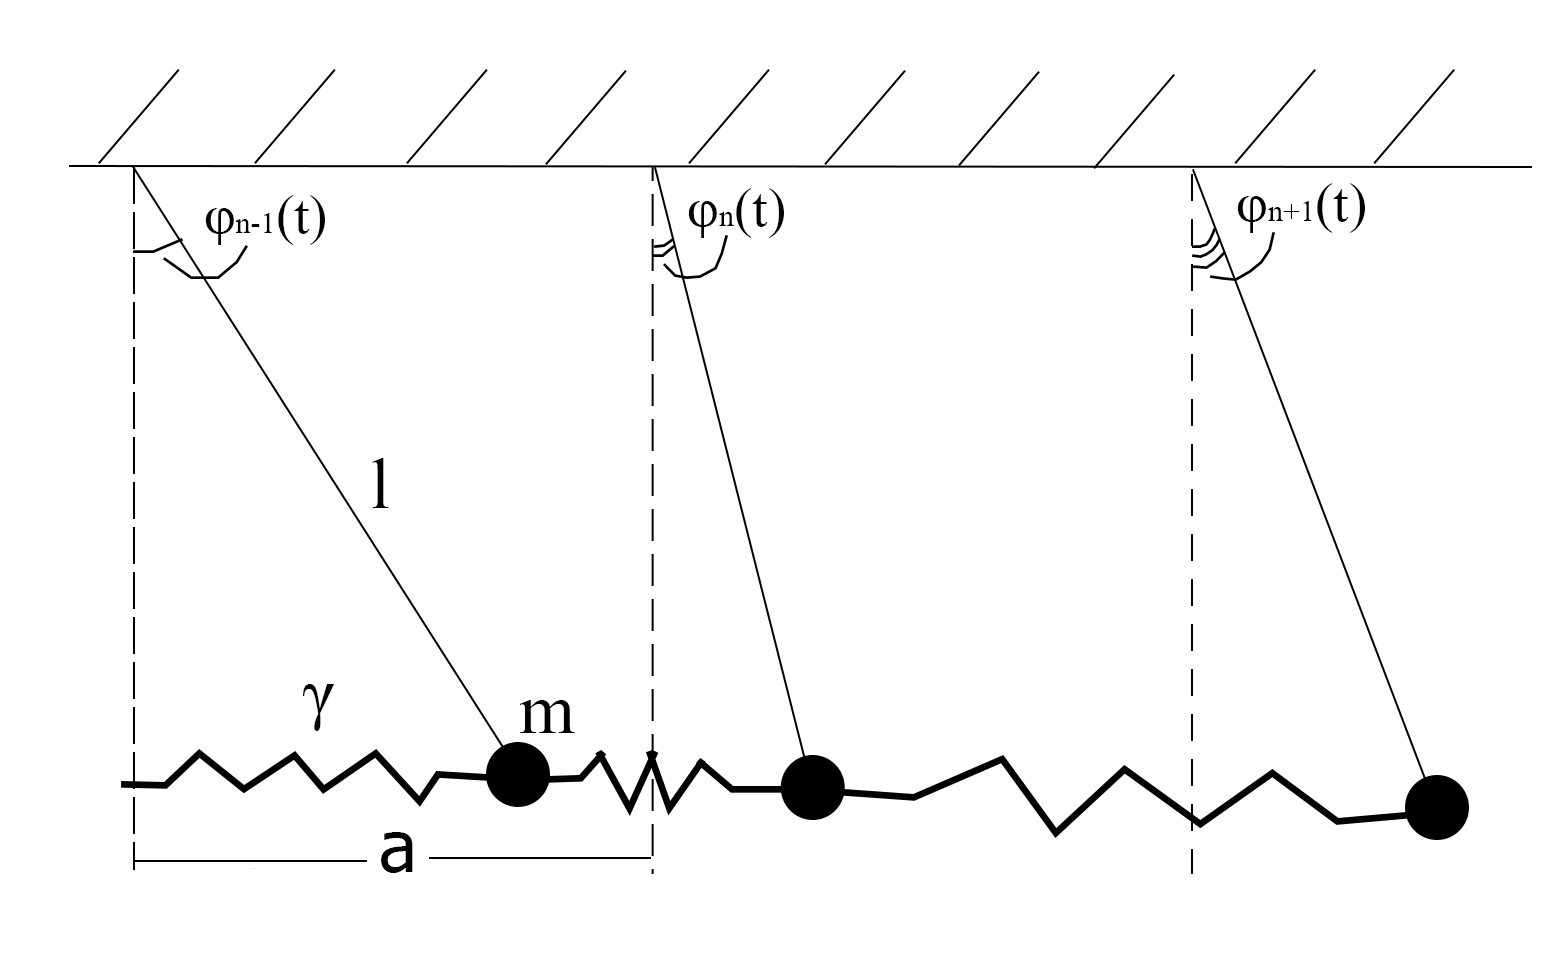
\includegraphics[width=0.5\linewidth]{fig/fig1.jpg}
	\label{fig:fig1}
\end{figure}

Состояние маятника зависит не только от времени t, но и от номера маятника n, т.е. n в некотором смысле играет роль пространственной координаты. Запишем уравнение динамики такого маятника:

\begin{equation}
	\ddot{\phi}_n+\omega^2_o \phi_n=\frac{\gamma}{m}[(\phi_{n-1}-\phi_n)+(\phi_{n+1}-\phi_n)].
	\label{eq:1}
\end{equation}

Каждый маятник действует на соседний, сила взаимодействия зависит от разности значений углов. Перепишем:

\begin{equation*}
	\ddot{\phi}_n+\omega^2_o \phi_n=\frac{\gamma}{m}[(\phi_{n-1}-2\phi_n+\phi_{n+1})].
\end{equation*}

Часто такую связь называют диффузионной, хотя, конечно, никакого отношения к процессу диффузии она не имеет. В системе нет диссипации, она линейна (нелинейность порождала бы новые частоты).

\begin{equation}
	\phi_n=A e^{i(\omega t-nka)}.
	\label{eq:2}
\end{equation}

Такая форма записи учитывает, что возмущение от маятника к маятнику проходит за некоторое конечное время.

\begin{equation*}
	-\omega^2+\omega_o^2=\frac{\gamma}{m}(e^{-ika}-2+e^{ika}),
\end{equation*}

\begin{equation}
	\omega^2=\omega_o^2-\frac{\gamma}{m}(e^{-ika}-2+e^{ika}).
	\label{eq:3}
\end{equation}

Рассмотрим случай \textit{k - действительное}
\begin{equation*}
	\omega^2=\omega_o^2-\frac{\gamma}{m}(-2+2\cos{ka}),
\end{equation*}

\begin{equation}
	\omega^2=\omega_o^2+\frac{4\gamma}{m}\sin^2{\frac{ka}{2}}.
	\label{eq:4}
\end{equation}

Установили, что $\omega$ и k связаны соотношением \eqref{eq:4}

\begin{figure}[H]
	\centering
	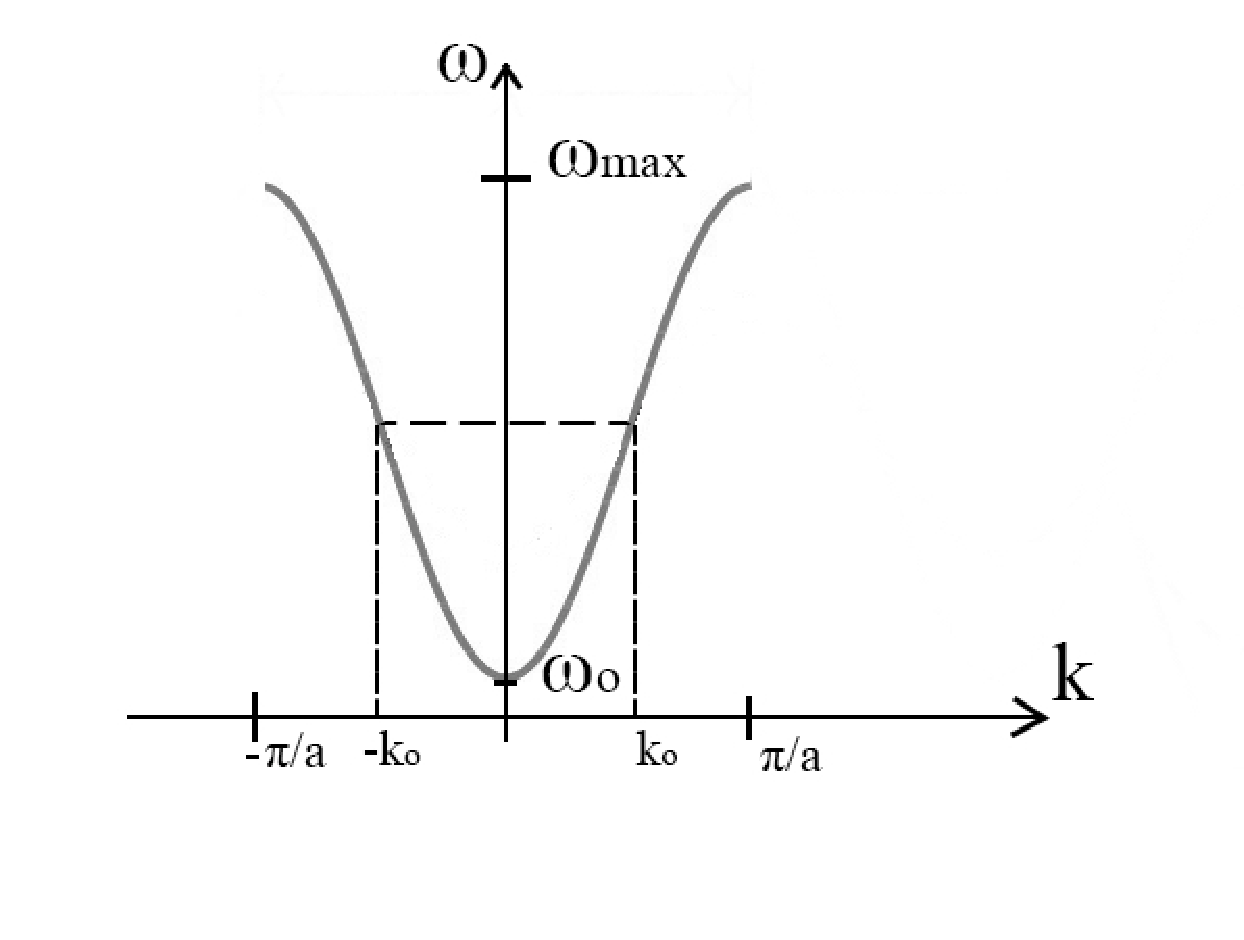
\includegraphics[width=0.5\linewidth]{fig/fig2.pdf}   
\end{figure}

\begin{equation*}
	\omega_{max}=\sqrt{\omega_o^2+\frac{4\gamma}{m}}.
\end{equation*}

Если $\omega_o < \omega < \omega_{max}$, то каждому $\omega$ соответствует $k_o$ и $-k_o$

Получим две гармонические бегущие волны:

\begin{equation*}
	\phi_n=A e^{i(\omega t+nk_oa)} ~~\text{и} ~~\phi_n=A e^{i(\omega t-nk_oa)},
\end{equation*}
где k - волновое число. Поскольку система линейна, любая линейная комбинация решений тоже будет решением. Диапазон $\omega_o < \omega < \omega_{max}$ называют полосой прозрачности (или полосой пропускания). Вне этой полосы решению не отвечают действительные k. В этом случае число \textit{k - чисто мнимое} (чисто - ибо нет диссипации в системе) и $k=i\kappa$:
\begin{equation}
	\omega^2=\omega_o^2-\frac{4\gamma}{m}\sh^2{\frac{\varkappa a}{2}},
	\label{eq:5}
\end{equation}
а $\phi_n=A e^{-n\varkappa a} e^{i\omega t}$ (при $n\rightarrow \infty$, $\phi_n \rightarrow 0$). В этих областях волна не проходит. 

Почему в одних случаях система пропускает волну, а в других нет?

Если мы находимся в полосе прозрачности, то $v_\text{фаз}=v_\text{фаз}(k), v_\text{фаз}=v_\text{фаз}(\omega)$. Если фазовая скорость зависит от частоты или волнового числа, то среда диспергирующая, а \eqref{eq:4} - дисперсионное соотношение. Дисперсия возникает из-за наличия собственных пространственно-временных масштабов (a и $\omega_o$). У каждой компоненты волнового пакета будет своя фазовая скорость, возникнет его деформация.

\subsection{Предельный переход от цепочной структуры в среде}
Введем пространственную координату $x$ вдоль балки. Сделаем замену, считая, что $\phi_n$ зависит от двух переменных:
\begin{gather*}
	\phi_n(t) \rightarrow \phi(x,t), \\
	\phi_{n+1}(t) \rightarrow \phi(x+a,t)=\phi(x,t)+\pdv{\phi}{x}a +\frac12 \pdv[2]{\phi}{x}a^2+\dots
\end{gather*}

Считая a малым, разложим в ряд по степеням a:

\begin{equation}
	\phi_{n-1}(t) \rightarrow \phi(x-a,t)=\phi(x,t)-\pdv{\phi}{x}a +\frac12 \pdv[2]{\phi}{x}a^2+\dots,
	\label{eq:6}
\end{equation}
и подставим в \eqref{eq:1}

\begin{gather*}
	\pdv[2]{\phi}{t} + \omega_o^2 \phi=\frac{\gamma}{m}a^2 \pdv[2]{\phi}{x}, \\
	\frac{\gamma}{m}a^2 = v^2,
\end{gather*}
\begin{equation}
	\pdv[2]{\phi}{t}-v^2\pdv[2]{\phi}{x}+\omega_o^2\phi=0 -\text{Уравнение Клейна-Гордона}.
	\label{eq:7}
\end{equation}

Уравнение \eqref{eq:7} не что иное, как уравнение в частных производных. Когда мы можем использовать \eqref{eq:7} вместо \eqref{eq:1}?

Предполагали, что
\begin{enumerate}
	\item $\phi_n$, определенная в точке, определена и между дискретными точками подвеса;
	\item отброшены величины третьего порядка;
	\item a-мало
\end{enumerate}

Построим дисперсионную характеристику для \eqref{eq:7}

\begin{gather*}
	\phi(x,t)=Ae^{i(\omega t + kx)}, \\ -\omega^2-k^2v^2+\omega_o^2=0,
\end{gather*}
\begin{equation}
	\omega^2 = \omega_o^2 + k^2v^2.
	\label{eq:8}
\end{equation}
\begin{figure}[H]
	\centering
	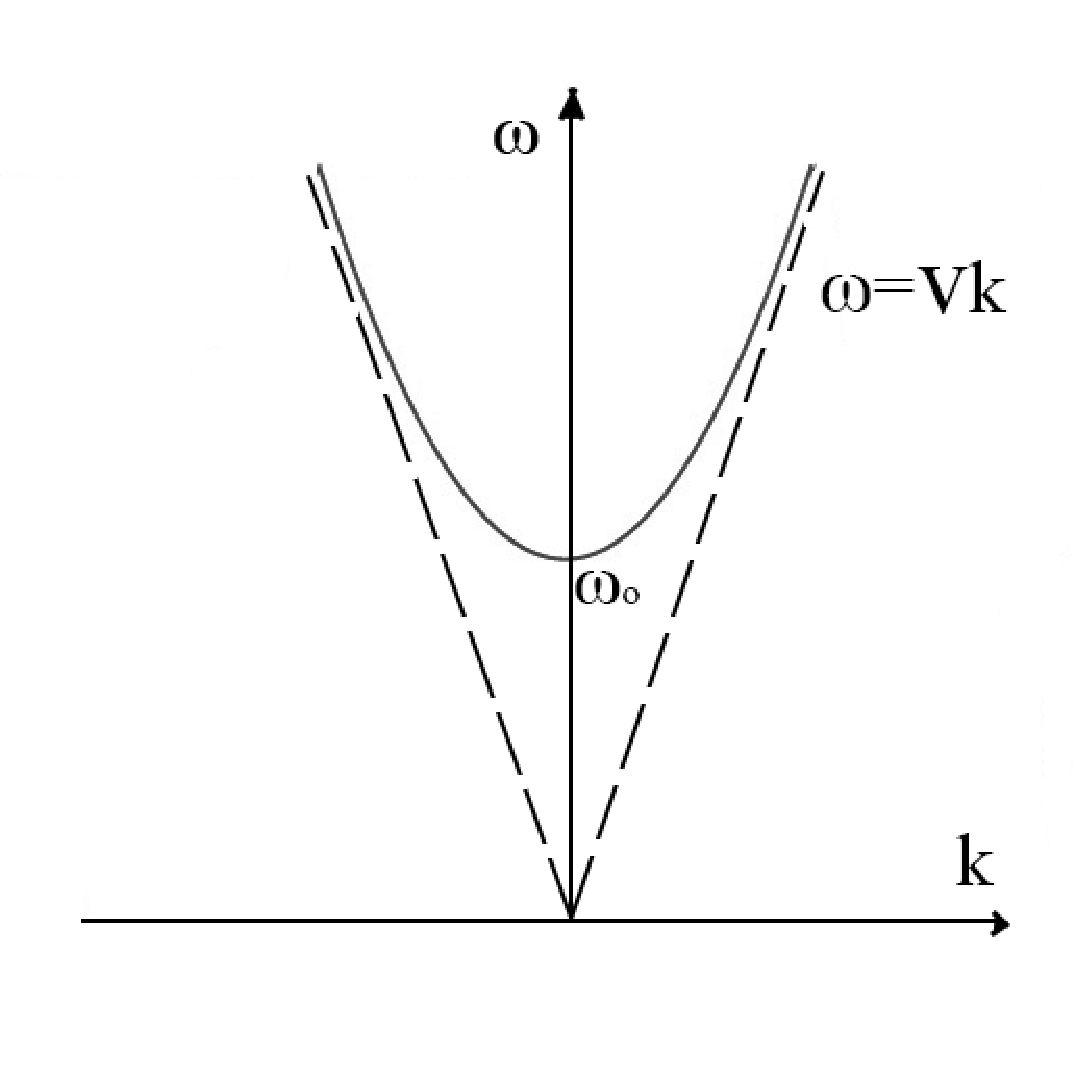
\includegraphics[width=0.5\linewidth]{fig/fig3.pdf}   
\end{figure}

Есть две асимптоты. 

При каких условиях дисперсионки совпадут?

$\lambda\gg a$ или $ka\ll$ - условие длинноволновой зоны, можно от одной перейти к другой, поскольку пространственный масштаб не сказывается, мы им пренебрегаем. Если $\omega_0 \rightarrow 0$, то из \eqref{eq:8}: $\omega^2=k^2v^2$. В этом случае система не обладает дисперсией. 

\begin{figure}[H]
	\centering
	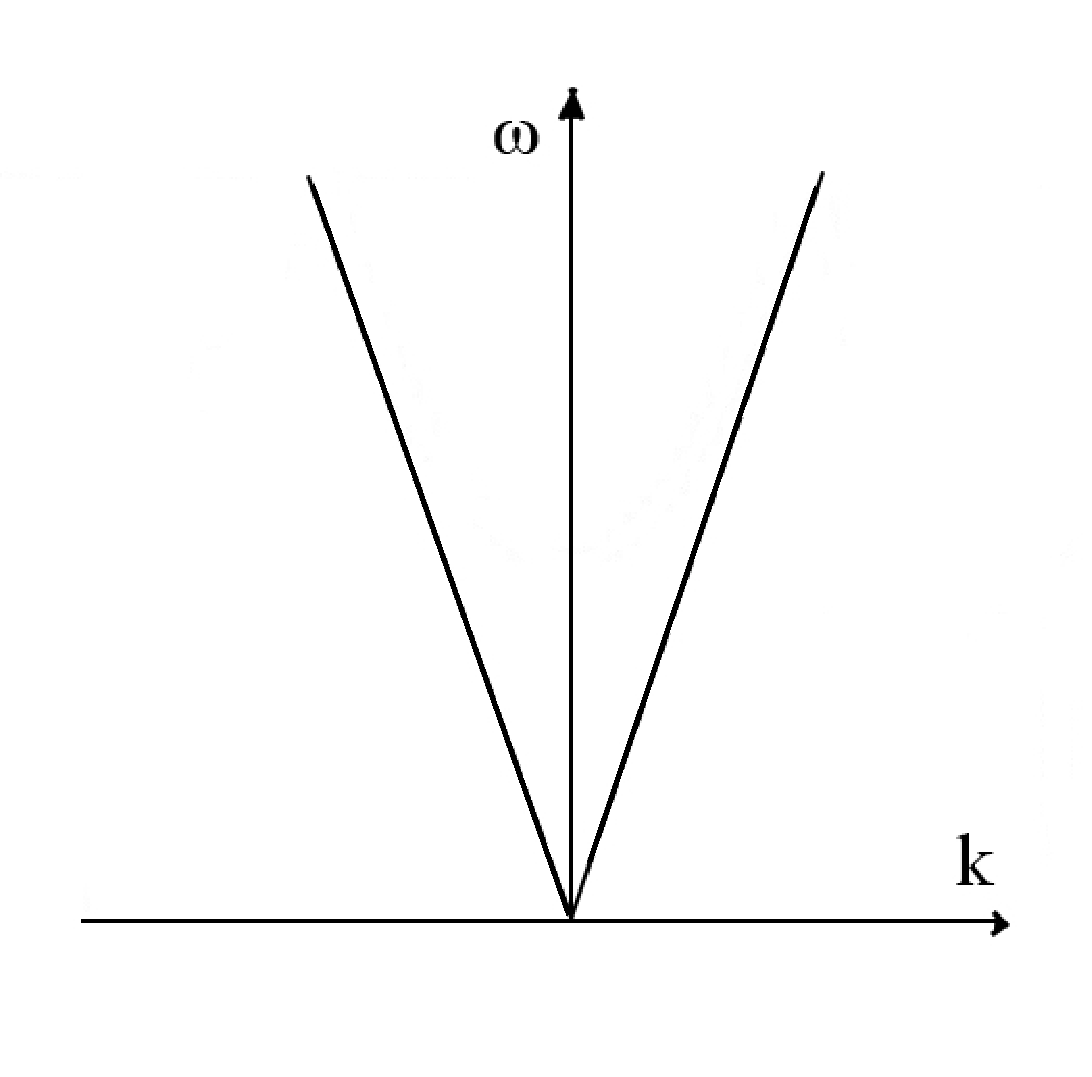
\includegraphics[width=0.5\linewidth]{fig/fig4.pdf}   
\end{figure}

Дисперсионная характеристика проявляется в области прозрачности/непрозрачности и зависимости $v_\text{фаз}$ от k или $\omega$.

Получили, шарики плотно друг к другу и покоятся.

Переход от цепочки к среде называется длинноволновым переходом. при нем теряется дискретность системы.

\subsection{Составление дисперсионного уравнения для произвольной линейной системы}

Рассмотрим многомерную систему
\begin{equation}
	A\pdv{\vec{U}}{t}+B\pdv{\vec{U}}{x}+C\vec{U}=0.
	\label{eq:9}
\end{equation}

A, B, C - $n\times n$ - матрицы; $\vec{U}(x,t)$ описывает состояние системы.

\begin{equation}
	\vec{U}=\vec{\phi} e^{i(\omega t - kx)}.
	\label{eq:10}
\end{equation}

\begin{equation*}
	\vec\phi=
	\begin{pmatrix}
		\phi_1 \\
		\phi_2 \\
		\phi_3 \\
		\vdots \\
		\phi_n \\
	\end{pmatrix}
	,
\end{equation*}

\begin{equation*}
	Ai\omega\vec\phi-iBk\vec\phi+C\vec\phi=0,
\end{equation*}
\begin{equation}
	(A\omega-Bk-iC)\vec\phi i=0.
	\label{eq:11}
\end{equation}

\eqref{eq:11} представляет собой систему линейных однородных уравнений относительно компонент вектора $\vec\phi$. Она имеет решение, если ее детерминант
\begin{equation}
	det(A\omega-Bk-iC)=0.
	\label{eq:12}
\end{equation}

для краткости обозначают $D(\omega,k)=0$. он связывает $\omega$ и k, т.е. задает дисперсионную характеристику. Следовательно, для $\forall k$ дисперсионное соотношение определяют n значений $\omega$: $\omega_1(k), \dots, \omega_n(k)$. Каждой паре k, $\omega_s(k)$ отвечает некоторый вектор, определяемый \eqref{eq:11}. При этом решением будут не только $k, \omega, \vec\phi$, но и $k^*, \omega^*, \vec\phi^*$. Можно построить действительное решение:
\begin{equation}
	\vec{U}(x,t)=\vec\phi e^{i(\omega t-kx)}+\vec\phi^* e^{-i(\omega^* t-k^*x)}.
	\label{eq:13}
\end{equation}

\eqref{eq:13} задает гармоническую волну, если $k, \omega$ действительные. Если же $k, \omega$ комплексные, то \eqref{eq:13} задает нарастающее или затухающее колебание. При этом общее решение может выть записано в виде 
\begin{equation*}
	\vec{U}(x,t)=\sum_{s=1}^{n} \phi^{(s)}e^{i(\omega_s(k)t-kx)} + \text{к.с}.
\end{equation*}

Как только будут учтены граничные условия, получится аналог характеристического уравнения.

\subsection{Влияние граничных условий}
Предположим, маятники были свернуты в кольцо, следовательно, должно уложиться целое число полуволн: 

\begin{gather*}
	n=1,\dots,N;~~\phi_{n-1}-2\phi_n+\phi_{n+1}; \\
	k=\frac{2\pi n}{l};~~\phi_{N+1}=\phi_1;~~k=k_n.
\end{gather*}	

Примером распределенной системы может служить струна длины l, концы которой закреплены:
\begin{figure}[H]
	\centering
	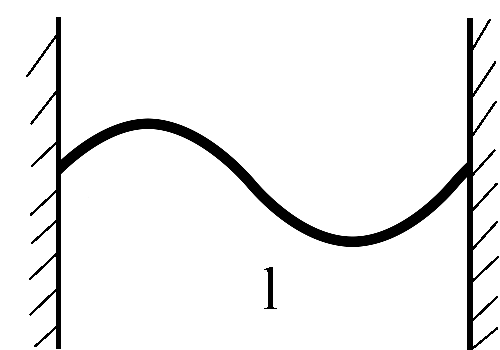
\includegraphics[width=0.5\linewidth]{fig/fig5.pdf}   
\end{figure}
\begin{gather*}
	U(x,t), \\ U(0,t)=u(l,t)=0, \\ U(x,t)=\phi_1 e^{i(\omega t-kx)}+\phi_2 e^{i(\omega t+kx)}, \\
	\begin{cases}
		\phi_1 e^{i\omega t}+\phi_2 e^{i\omega t}=0 \\
		\phi_1 e^{i\omega t}+\phi_2 e^{i\omega t+ikl}=0
	\end{cases}
	\\ \phi_1=-\phi_2,~~ \sin{kl}=0,~~ k=\frac{\pi n}{l}=k_n
\end{gather*}

\begin{equation}
	\begin{cases}
		D(\omega,k)=0 \\
		k=k_n
	\end{cases}
	\label{eq:14}
\end{equation}

Отсюда следует, что $\omega=omega_n$. Если среда без дисперсии, то спектры волновых чисел и волновых частот будут эквидистантными. 

\subsection{Устойчивость состояний равновесия нелинейных распределенных систем}
Простейшим типом решений распределенных систем являются такие состояния, которые не меняются ни во времени, ни в пространстве: $U(x,t); U=U_o=const$.
\begin{equation}
	\pdv{U}{t}=f(U)+D\pdv[2]{U}{x},
	\label{eq:15}
\end{equation}
где $f(U)$ - нелинейная функция. Пусть, кубическая. Если убрать D. то уравнение будет описывать динамику точки в среде.
\begin{figure}[H]
	\centering
	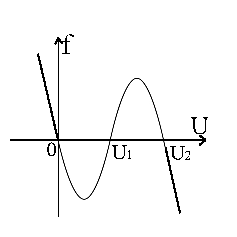
\includegraphics[width=0.5\linewidth]{fig/fig6.pdf}   
\end{figure}

Три точки, где $f(U)=0$. В системе могут быть стационарные решения (не зависящие от времени) - это другой тип решения. Будем рассматривать их решение в классе гармонических функций. 
\begin{equation*}
	\xi(x,t) \sim e^{pt+ikx}
\end{equation*}

Линеаризуем \eqref{eq:15} на состояниях равновесия:
\begin{equation*}
	U=U^*+\xi(x,t),
\end{equation*}
\begin{equation}
	\pdv{\xi}{t}=D\pdv[2]{\xi}{x}+f'(U^*)\xi(x,t).
	\label{eq:16}
\end{equation}
\begin{gather*}
	f(U^*+\xi(x,t))\approx f(U^*)+f'(U^*)\cdot\xi(x,t), \\ \xi(x,t)=A e^{pt+ikx} \\
	p =-Dk^2+f'(U^*), \\ U=0,~~U=U_2,~~f'(U^*)<0.
\end{gather*}

Для каждого А.
\begin{figure}[H]
	\centering
	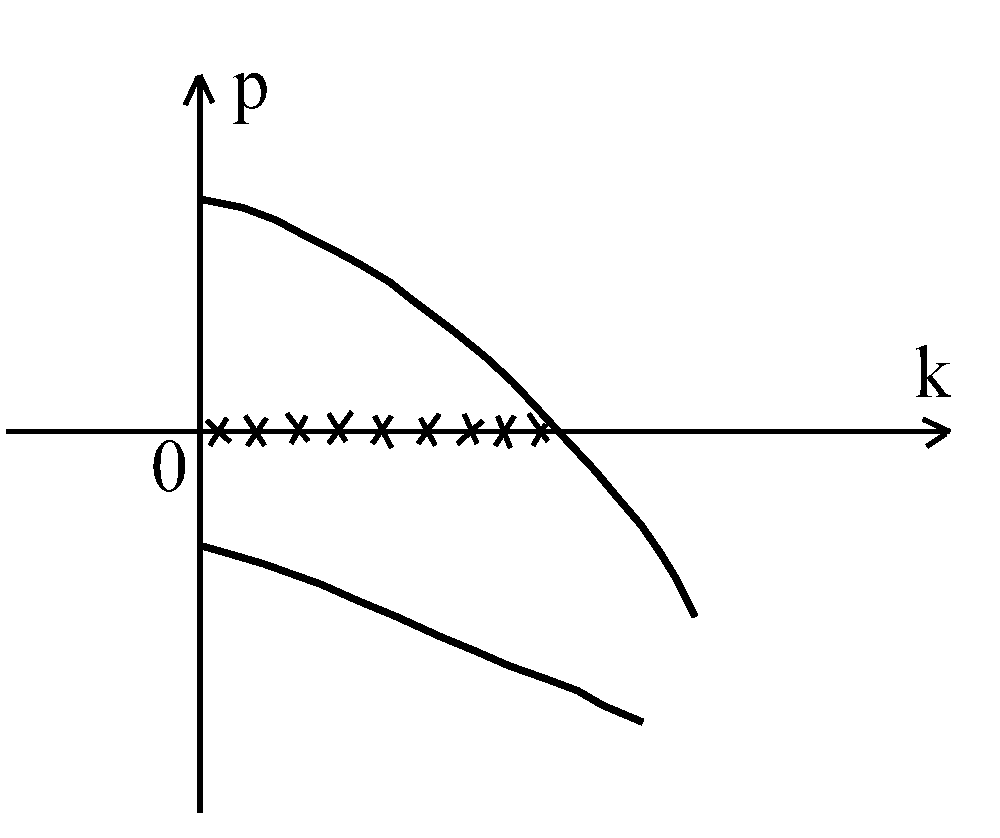
\includegraphics[width=0.5\linewidth]{fig/fig7.pdf}   
\end{figure}

Все решения такого вида затухают, следовательно, $U=0, U=U_2$ устойчивые, а $U_1$ - неустойчивое в классе возмущений $\xi(x,t)=A e^{pt+ikx}$.

В частности, \eqref{eq:15}, описывает распространение пламени по бикфордовому (огнепроводному) шнуру. Волна превращает вещество из несгоревшего материала в сгоревшее.


\section{15.04.19 Диффузионная неустойчивость. Структура Тьюринга}
Многие биологические объекты обладают периодической структурой. Например, зебра, дождевой червь, сороконожка. Однако известно, что изначально, при появлении, они однородны. Рассмотрим одномерный случай структур.

Тьюринг предположил, что существуют два вещества. Одно из них - $U(x,t)$ - стимулирует рост клеток. Его назвали активатором. Другое - $V(x,t)$ - замедляет рост. Это ингибитор. Следующим предположением было наличие некоторых химических реакций и присутствие диффузии. Фактически, Тьюринг записал уравнение реакции диффузии. 
\begin{equation}
\begin{cases}
		\pdv{U}{t}=f(U,V)+D_1 \pdv[2]{U}{x} \\
		\pdv{V}{t}=g(U,V)+D_2 \pdv[2]{V}{x},
	\end{cases}	\
	\label{eq:17}
\end{equation}
где $f,g$  - это некоторые нелинейные функции.

Эта система двухкомпонентная, произвольная координата одна. Предположим, \eqref{eq:17} имеет состояние равновесия, т.е. существует решение системы
\begin{equation}
\begin{cases}
		f(U,V)=0 \\
		g(U,V)=0.
	\end{cases}	\
	\label{eq:18}
\end{equation}
$U=U_0, V=V_0$.

Исследуем на устойчивость. Положим,
\begin{gather*}
	U=U_0+\xi(x,t) \\
	V=V_0+\eta(x,t).
\end{gather*}

Линеаризуем (оставляем только линейную часть):
\begin{equation}
	\begin{cases}
		\pdv{\xi}{t}=f'_u(U_0, V_0)\xi(x,t)+f'_v(U_0, V_0)\eta(x,t)+D_1 \pdv[2]{\xi(x,t)}{x} \\
		\pdv{\eta}{t}=g'_u(U_0, V_0)\xi(x,t)+g'_v(U_0, V_0)\eta(x,t)+D_2 \pdv[2]{\eta(x,t)}{x}.
	\end{cases}	
	\label{eq:19}
\end{equation}

Получили уравнения в частных производных. Будем искать решение в виде:
\begin{equation}
	\xi(x,t)=A e^{pt+ikx};~~\eta(x,t)=B e^{pt+ikx}.
	\label{eq:20}
\end{equation}

Подставляя эти решения и учитывая, что $f'$ и $g'$ - это производные в точке, т.е. константы, получим:
\begin{equation}
	\begin{cases}
		\pdv{\xi}{t}=a\xi+b\eta+D_1 \pdv[2]{\xi}{x} \\
		\pdv{\eta}{t}=c\xi+d\eta+D_2 \pdv[2]{\eta}{x},
	\end{cases}	
	\label{eq:21}
\end{equation}
где
\begin{gather*}
	a=f'_u(U_0, V_0),~~b=f'_v(U_0, V_0),~~c=g'_u(U_0, V_0),~~d=g'_v(U_0, V_0).
\end{gather*}

\begin{equation}
	\begin{cases}
		Ap=aA+bB-k^2 D_1A \\
		Bp=cA+dB-k^2 D_2A,
	\end{cases}	
	\label{eq:22}
\end{equation}

\eqref{eq:17} представляет собой систему линейных однородных уравнений относительно констант А,В. Она имеет нетривиальное решение, если ее определитель не равен нулю. Раскрывая определитель, получим характеристическое уравнение для p:
\begin{equation}
	p^2+(D_2k^2+D_1k^2-a-d)p+(D_1k^2-a)(D_2k^2-d)-bc=0.
	\label{eq:23}
\end{equation}

Предположим, что в начальный момент $D_1=D_2=0$, тогда
\begin{equation}
	p^2-(a+d)p+ad-bc=0.
	\label{eq:24}
\end{equation}

Сначала структуры у животных нет, следовательно, без диффузии имеем устойчивое равновесие. Запишем условие для этого:
\begin{gather*}
	\Delta_o=ad-bc>0, \\ \sigma_0=a+d<0,
\end{gather*}
тогда состояние равновесия будет устойчивым. 

\begin{figure}[H]
	\centering
	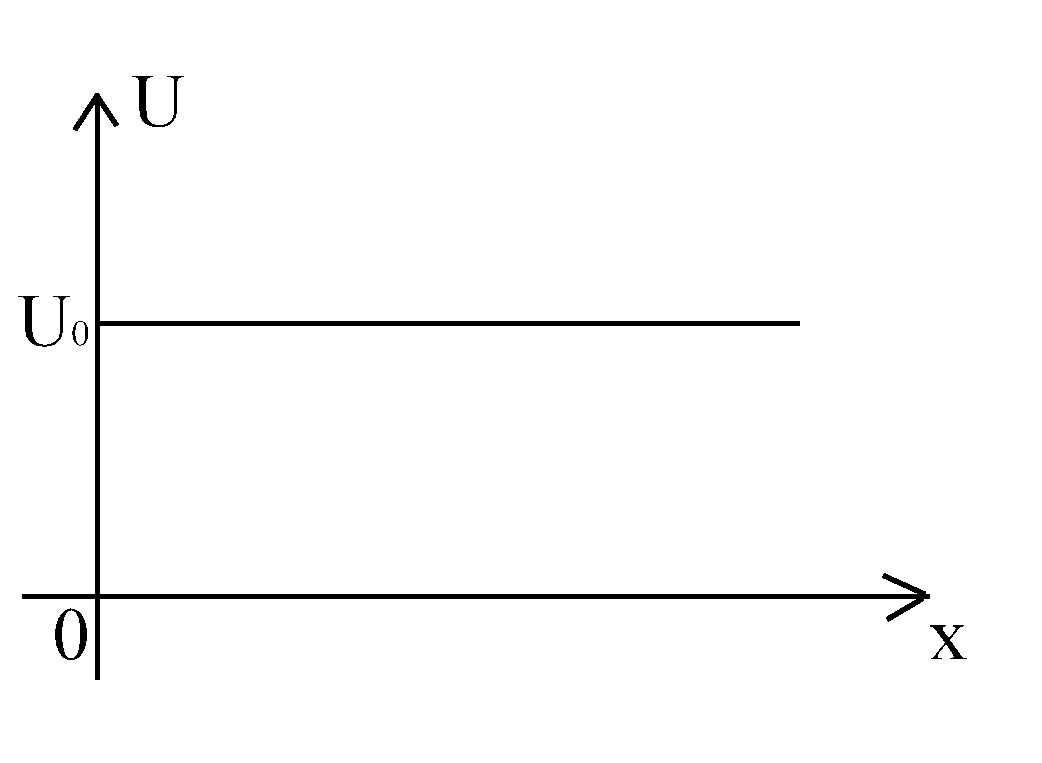
\includegraphics[width=0.5\linewidth]{fig/fig8.pdf}   
\end{figure}

По оси х U(активатор) и V(ингибитор) постоянны. 

Пусть теперь $D_1, D_2 \neq 0$. В этом случае \eqref{eq:24} после преобразований примет вид:
\begin{equation*}
	p^2-\sigma p+\Delta=0,
\end{equation*}
где
\begin{gather*}
	\Delta=a+d-(D_1+D_2)k^2=\sigma_0-(D_1+D_2)k^2, \\ \sigma=ad-bc-(aD_2+dD_1)k^2+D_1D_2k^4=\Delta_0-(aD_2+dD_1)k^2+D_1D_2k^4.
\end{gather*}

$Re\{p\}$ зависит от k. Анализ показывает:
\begin{figure}[H]
	\centering
	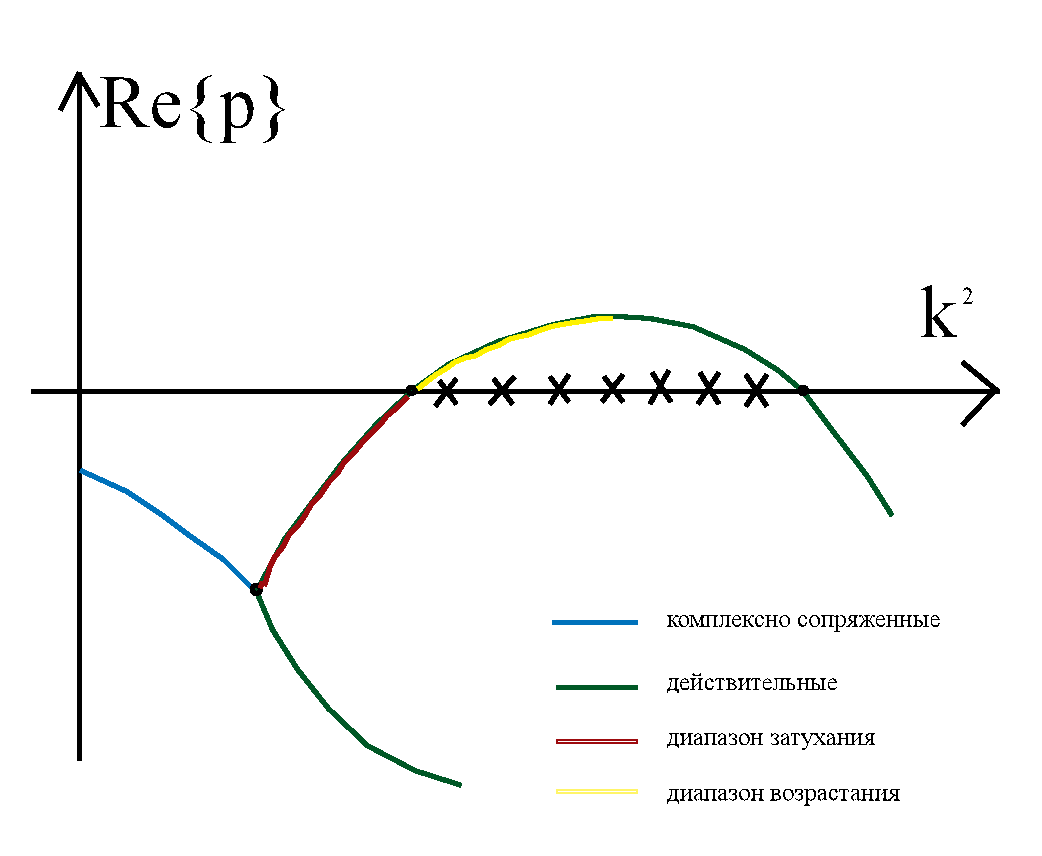
\includegraphics[width=0.5\linewidth]{fig/fig9.pdf}   
\end{figure}

Есть диапазон, где произошла потеря устойчивости состояния равновесия за счет действия диффузии. Это называется диффузионной неустойчивостью. Возникает аналог бифуркации Андронова-Хопфа. В диапазоне затухания все моды затухают, а возрастания - возрастают. Возникает периодическое по пространственной координате решение. Кроме того, оно пространственно неоднородное.  
\begin{figure}[H]
	\centering
	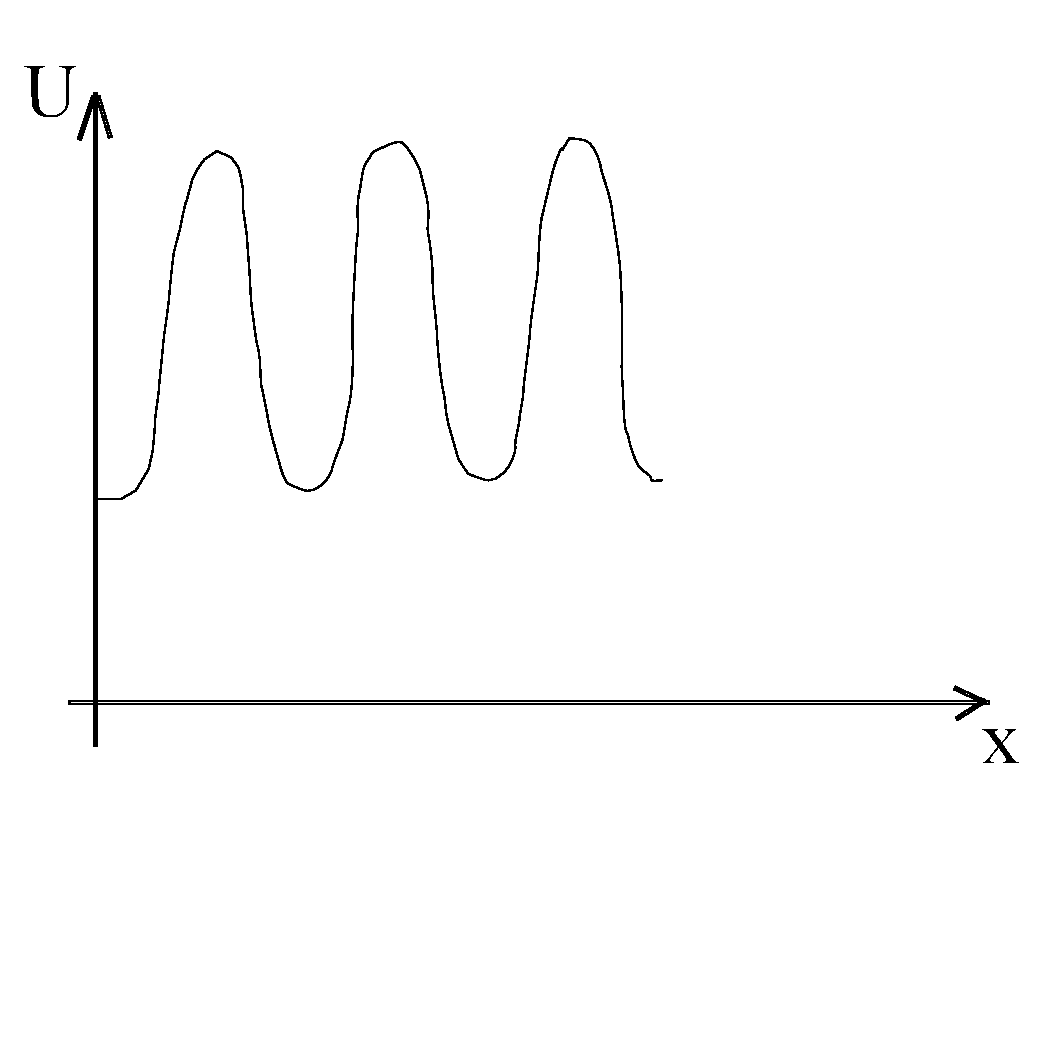
\includegraphics[width=0.5\linewidth]{fig/fig10.pdf}   
\end{figure}

Динамическая структура, обладающая свойством структурной устойчивости, иногда называется диссипативной структурой. Возникает за счет баланса. 

\subsection{Простые волны. Образование разрывов.}
Рассмотрим равномерную среду, свойства которой описывает скалярная функция $U(x,t)$. Среда линейная, без дисперсия. В таких средах возможно существование волновых движений, при этом все переменные описываются одинаковыми уравнениями:
\begin{equation}
	\pdv{U_j}{t}+V\pdv{U_j}{x}=0.
	\label{eq:25}
\end{equation}

В среде нет собственных масштабов и нелинейностей. V-const. В этой среде возможно существование так называемых римановых волн. 
\begin{equation}
	U_j=\phi(x-Vt),
	\label{eq:26}
\end{equation}
где $\phi$ - произвольная, обязательно дифференцируемая, функция.

Введем бегущую координату:
\begin{gather*}
	\xi=x-Vt, \\ \dv{\phi}{\xi} \pdv{\xi}{t}+V\dv{\phi}{\xi} \pdv{\xi}{x}=0, \\ -V\dv{\phi}{\xi}+V\dv{\phi}{\xi} \equiv 0.
\end{gather*}

\eqref{eq:26} является решением такой системы. 

Теперь рассмотрим нелинейную среду (но все еще без дисперсии). В таких средах могут существовать волны, которые обладают следующим свойством: переменные связаны алгебраически (если есть $U_1$ и $U_2$, то $U_3$ всегда можно пересчитать).

Рассмотрим пример: волны на мелкой воде. Гравитационные волны вдоль оси x.
\begin{figure}[H]
	\centering
	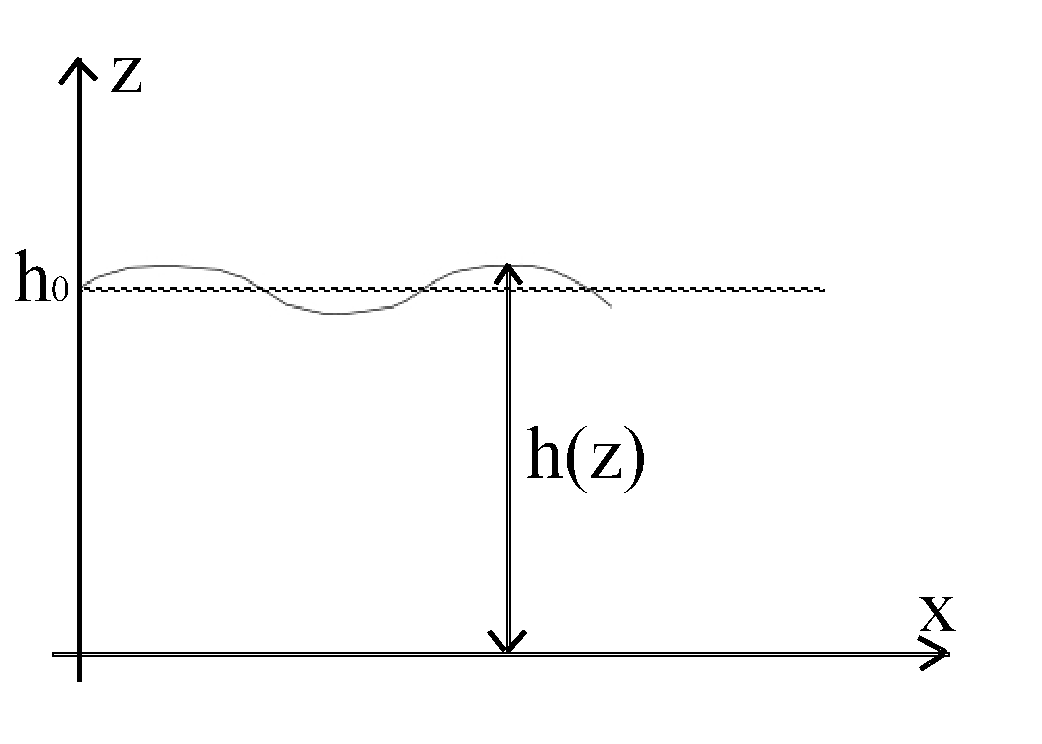
\includegraphics[width=0.4\linewidth]{fig/fig11.pdf}   
\end{figure}
$\lambda \gg h_0$

Состояние жидкости описывается: V - скоростью волны, h - профилем. Поскольку волны длинные, считаем, что $V\neq V(z)$.

Используем уравнение Эйлера: 
\begin{gather*}
	\pdv{V}{t}+V\pdv{V}{x}+\frac1{\rho}\pdv{\rho}{x}=0, \\ \rho=const, p-\text{среднее по высоте}, \\ \frac1{\rho}\pdv{\rho}{x}=g\pdv{h}{x}.
\end{gather*}

Давление больше там, где выше жидкость.
\begin{equation}
	\pdv{V}{t}+V\pdv{V}{x}+g\pdv{h}{x}=0.
	\label{eq:27}
\end{equation}

Добавим уравнение непрерывности:
\begin{gather*}
	\pdv{p}{t}+\pdv{(Vh)}{x}=0. 
\end{gather*}

Скорость изменения высоты слоя связана с разностью потока через x и dx
\begin{equation}
	\pdv{h}{t}+V\pdv{h}{x}+h\pdv{V}{x}=0.
	\label{eq:28}
\end{equation}

Предположим, h и V не являются независимыми переменными и $h=h(V)$.

Из уравнения \eqref{eq:27}: 
\begin{gather*}
	\pdv{h}{x}=\dv{h}{V}\pdv{V}{x}, \\ \pdv{V}{t}+V\pdv{V}{x}+g\pdv{h}{x} = 0 ~(*).
\end{gather*}

Из уравнения \eqref{eq:28}:
\begin{gather*}
	\dv{h}{V}\pdv{V}{t}+V\dv{h}{V}\pdv{V}{x}+h(V)\pdv{V}{x} = 0, \\ \pdv{V}{t}+V\pdv{V}{x}+\frac{h(V)}{\dv{h}{V}}\pdv{h}{x} = 0 ~(**).
\end{gather*}

(*) и (**) должны совпадать, т.к описывают одну и ту же величину. 
\begin{equation*}
	g\dv{h}{V}=\frac{h}{\dv{h}{V}}~ \text{или} ~(\dv{h}{V})^2=\frac{h}{g} - \text{уравнение для нахождения h}.
\end{equation*}

\begin{gather*}
	\dv{h}{V}=\pm \sqrt{\frac{h(V)}{g}}, \\ \pdv{V}{t}+V\pdv{V}{x}\pm \sqrt{h(V)g} \pdv{V}{x} = 0.
\end{gather*}
\begin{equation}
	\pdv{V}{t}+(V\pm \sqrt{h(V)g})\pdv{V}{x} = 0
	\label{eq:29}
\end{equation}
- уравнение простой волны, которое в общем виде выглядит:
\begin{equation}
	\pdv{U}{t}+V(U)\pdv{U}{x} = 0
	\label{eq:30}
\end{equation}

Это уравнение справедливо не только на мелкой воде. Здесь $V$ - это функция среды.

Будем искать решение в виде:
\begin{equation}
	U = \phi(x-V(U)t),
	\label{eq:31}
\end{equation}
\begin{gather*}
	\xi=x-V(U)t.
\end{gather*}

Убедимся, что \eqref{eq:30} - решение:
\begin{gather*}
	\pdv{U}{t}=\dv{\phi}{\xi}\pdv{\xi}{t}=\dv{\phi}{\xi}\qty(-V(U)-t\dv{V}{U}\pdv{U}{t}), \\ \pdv{U}{t}\qty(1+\dv{\phi}{\xi}\dv{V}{U}t)=-V(U)\dv{\phi}{\xi},
\end{gather*}
\begin{equation}
	\pdv{U}{t}=-V(U)\dv{\phi}{\xi} \frac{1}{(1+\dv{\phi}{\xi}\dv{V}{U}t)}
	\label{eq:32}
\end{equation}
\begin{gather*}
	\pdv{U}{x}=\dv{\phi}{\xi} \frac{1}{(1+\dv{\phi}{\xi}\dv{V}{U}t)}
\end{gather*}

Для определенности:
\begin{figure}[H]
	\centering
	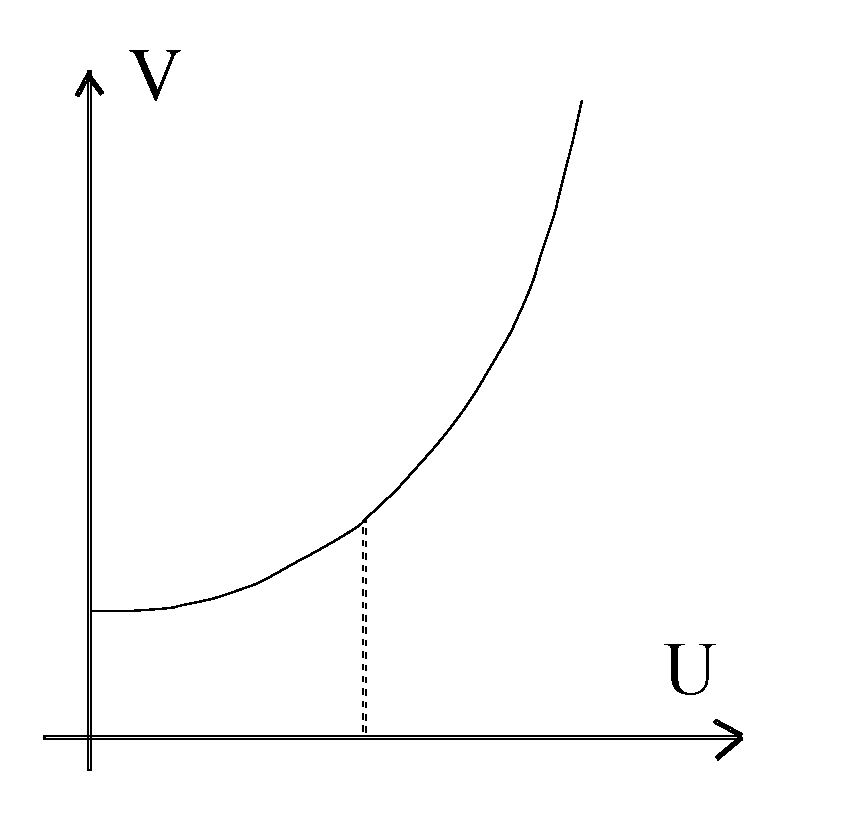
\includegraphics[width=0.4\linewidth]{fig/fig12.pdf}   
\end{figure}

У максимального значения U скорость наибольшая. Задается профиль $\phi$ при $t=0$:
\begin{figure}[H]
	\centering
	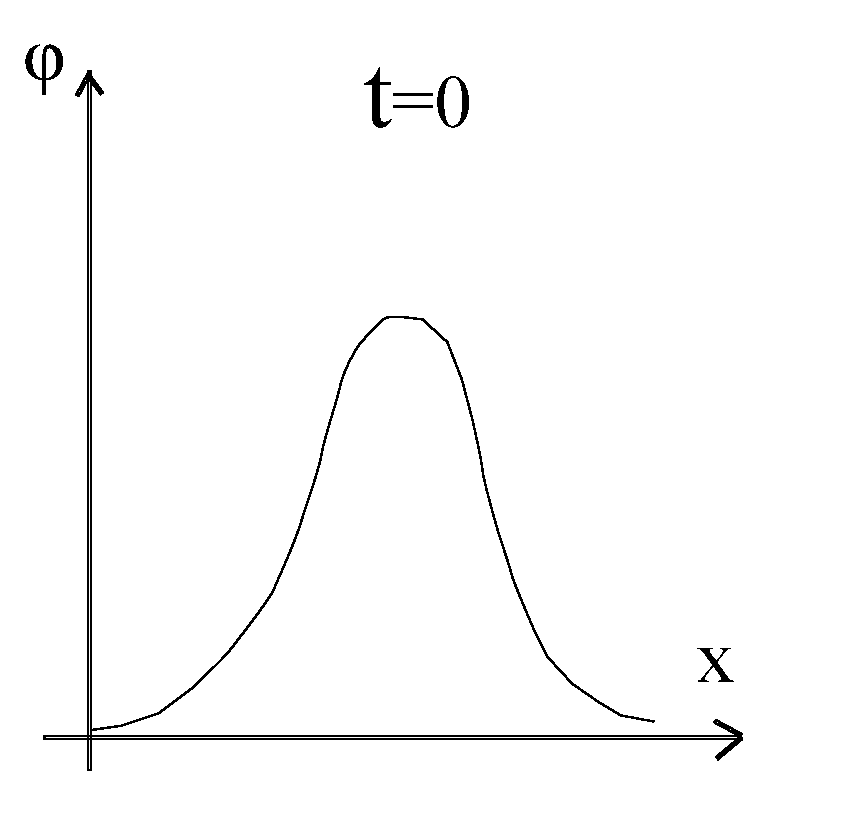
\includegraphics[width=0.4\linewidth]{fig/fig13.pdf}   
\end{figure}
или при $x=0$:
\begin{figure}[H]
	\centering
	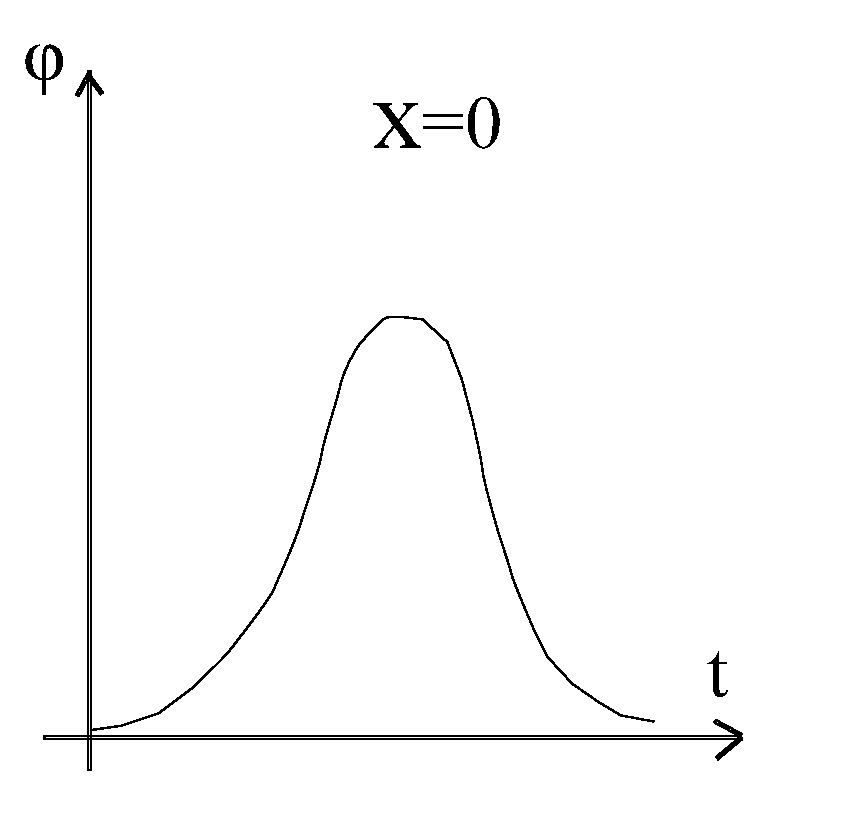
\includegraphics[width=0.4\linewidth]{fig/fig14.pdf}   
\end{figure}

Во время распространения, верх волны обгонит, произойдет укручение фронта, волна деформируется. 
\begin{figure}[H]
	\centering
	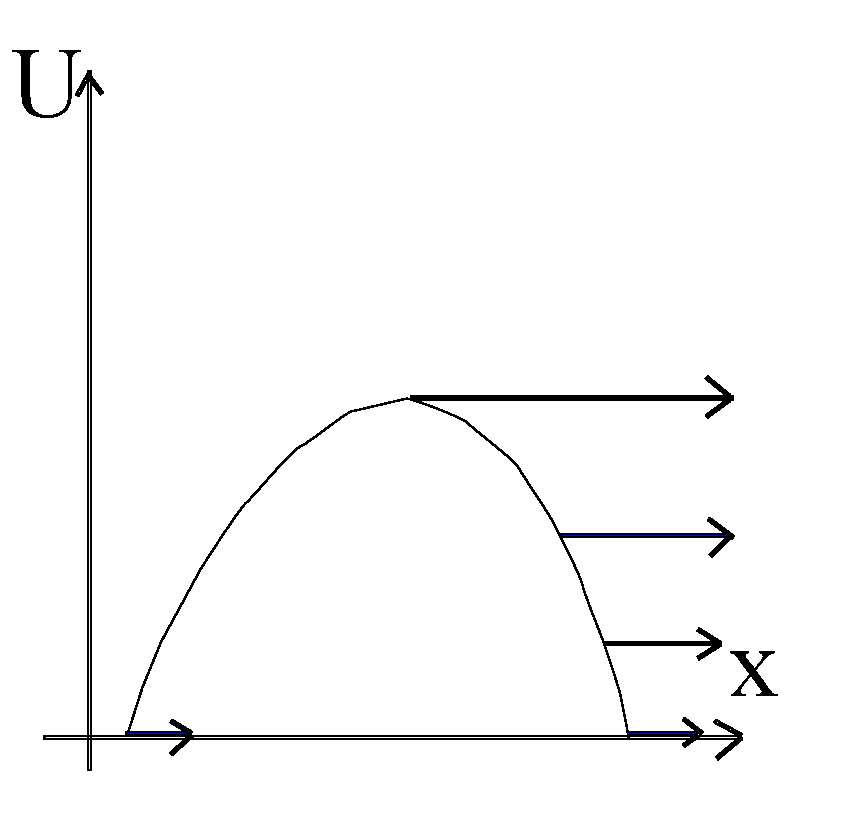
\includegraphics[width=0.4\linewidth]{fig/fig15.pdf}   
\end{figure}
\begin{figure}[H]
	\centering
	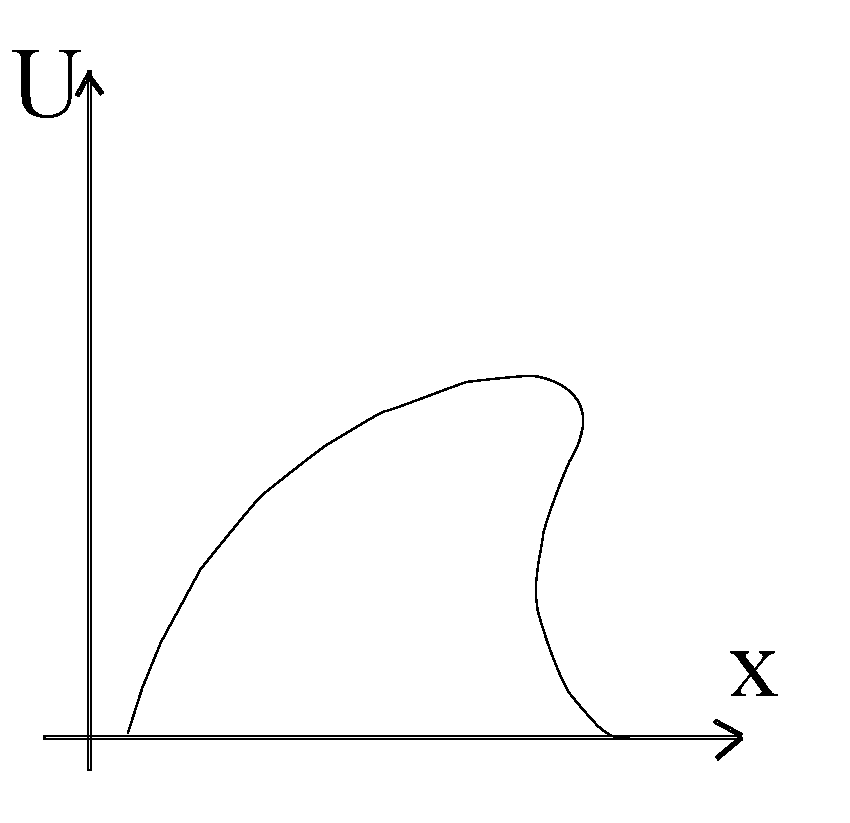
\includegraphics[width=0.4\linewidth]{fig/fig16.pdf}   
\end{figure}
\begin{figure}[H]
	\centering
	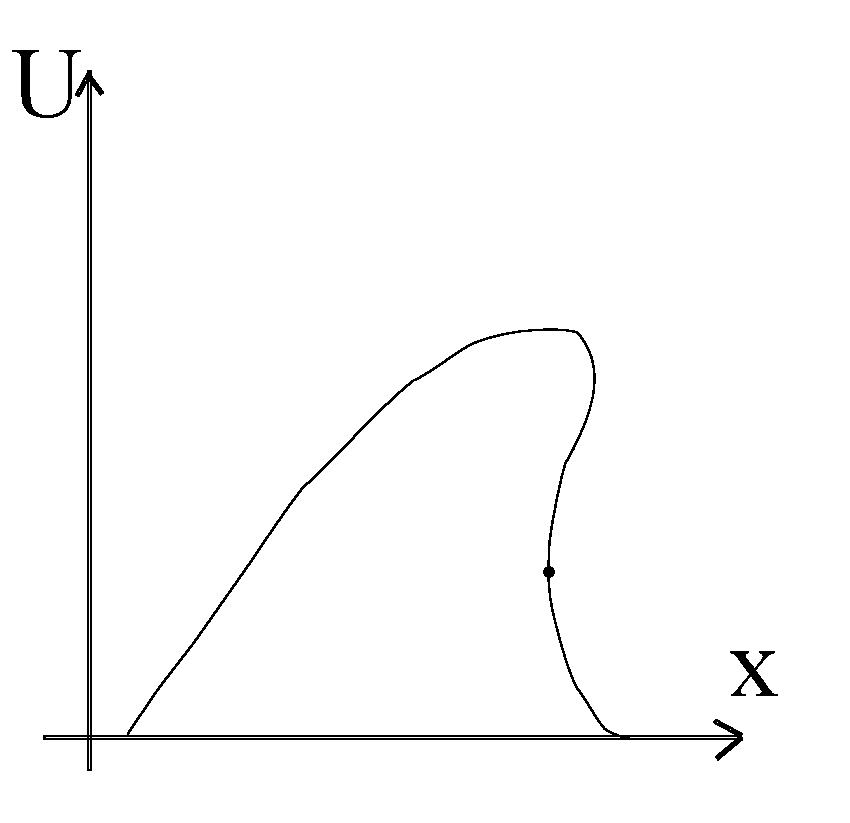
\includegraphics[width=0.4\linewidth]{fig/fig17.pdf}   
\end{figure}

Появится точка, где производные $\pdv{U}{t}, \pdv{U}{x} \rightarrow \infty $. Образуется бесконечный градиент и разрыв, который характеризуется состоянием $U^*, t^*, x^*$, его описание в рамках простой волны несправедливо. Вторые производные тоже обращаются в бесконечность, и точки эти можно найти.

\section{Солитоны в уравнении Кортевега - де Фриза} 
Рассмотрим узкий бассейн с жидкостью (должен быть достаточно длинным):
\begin{figure}[H]
	\centering
	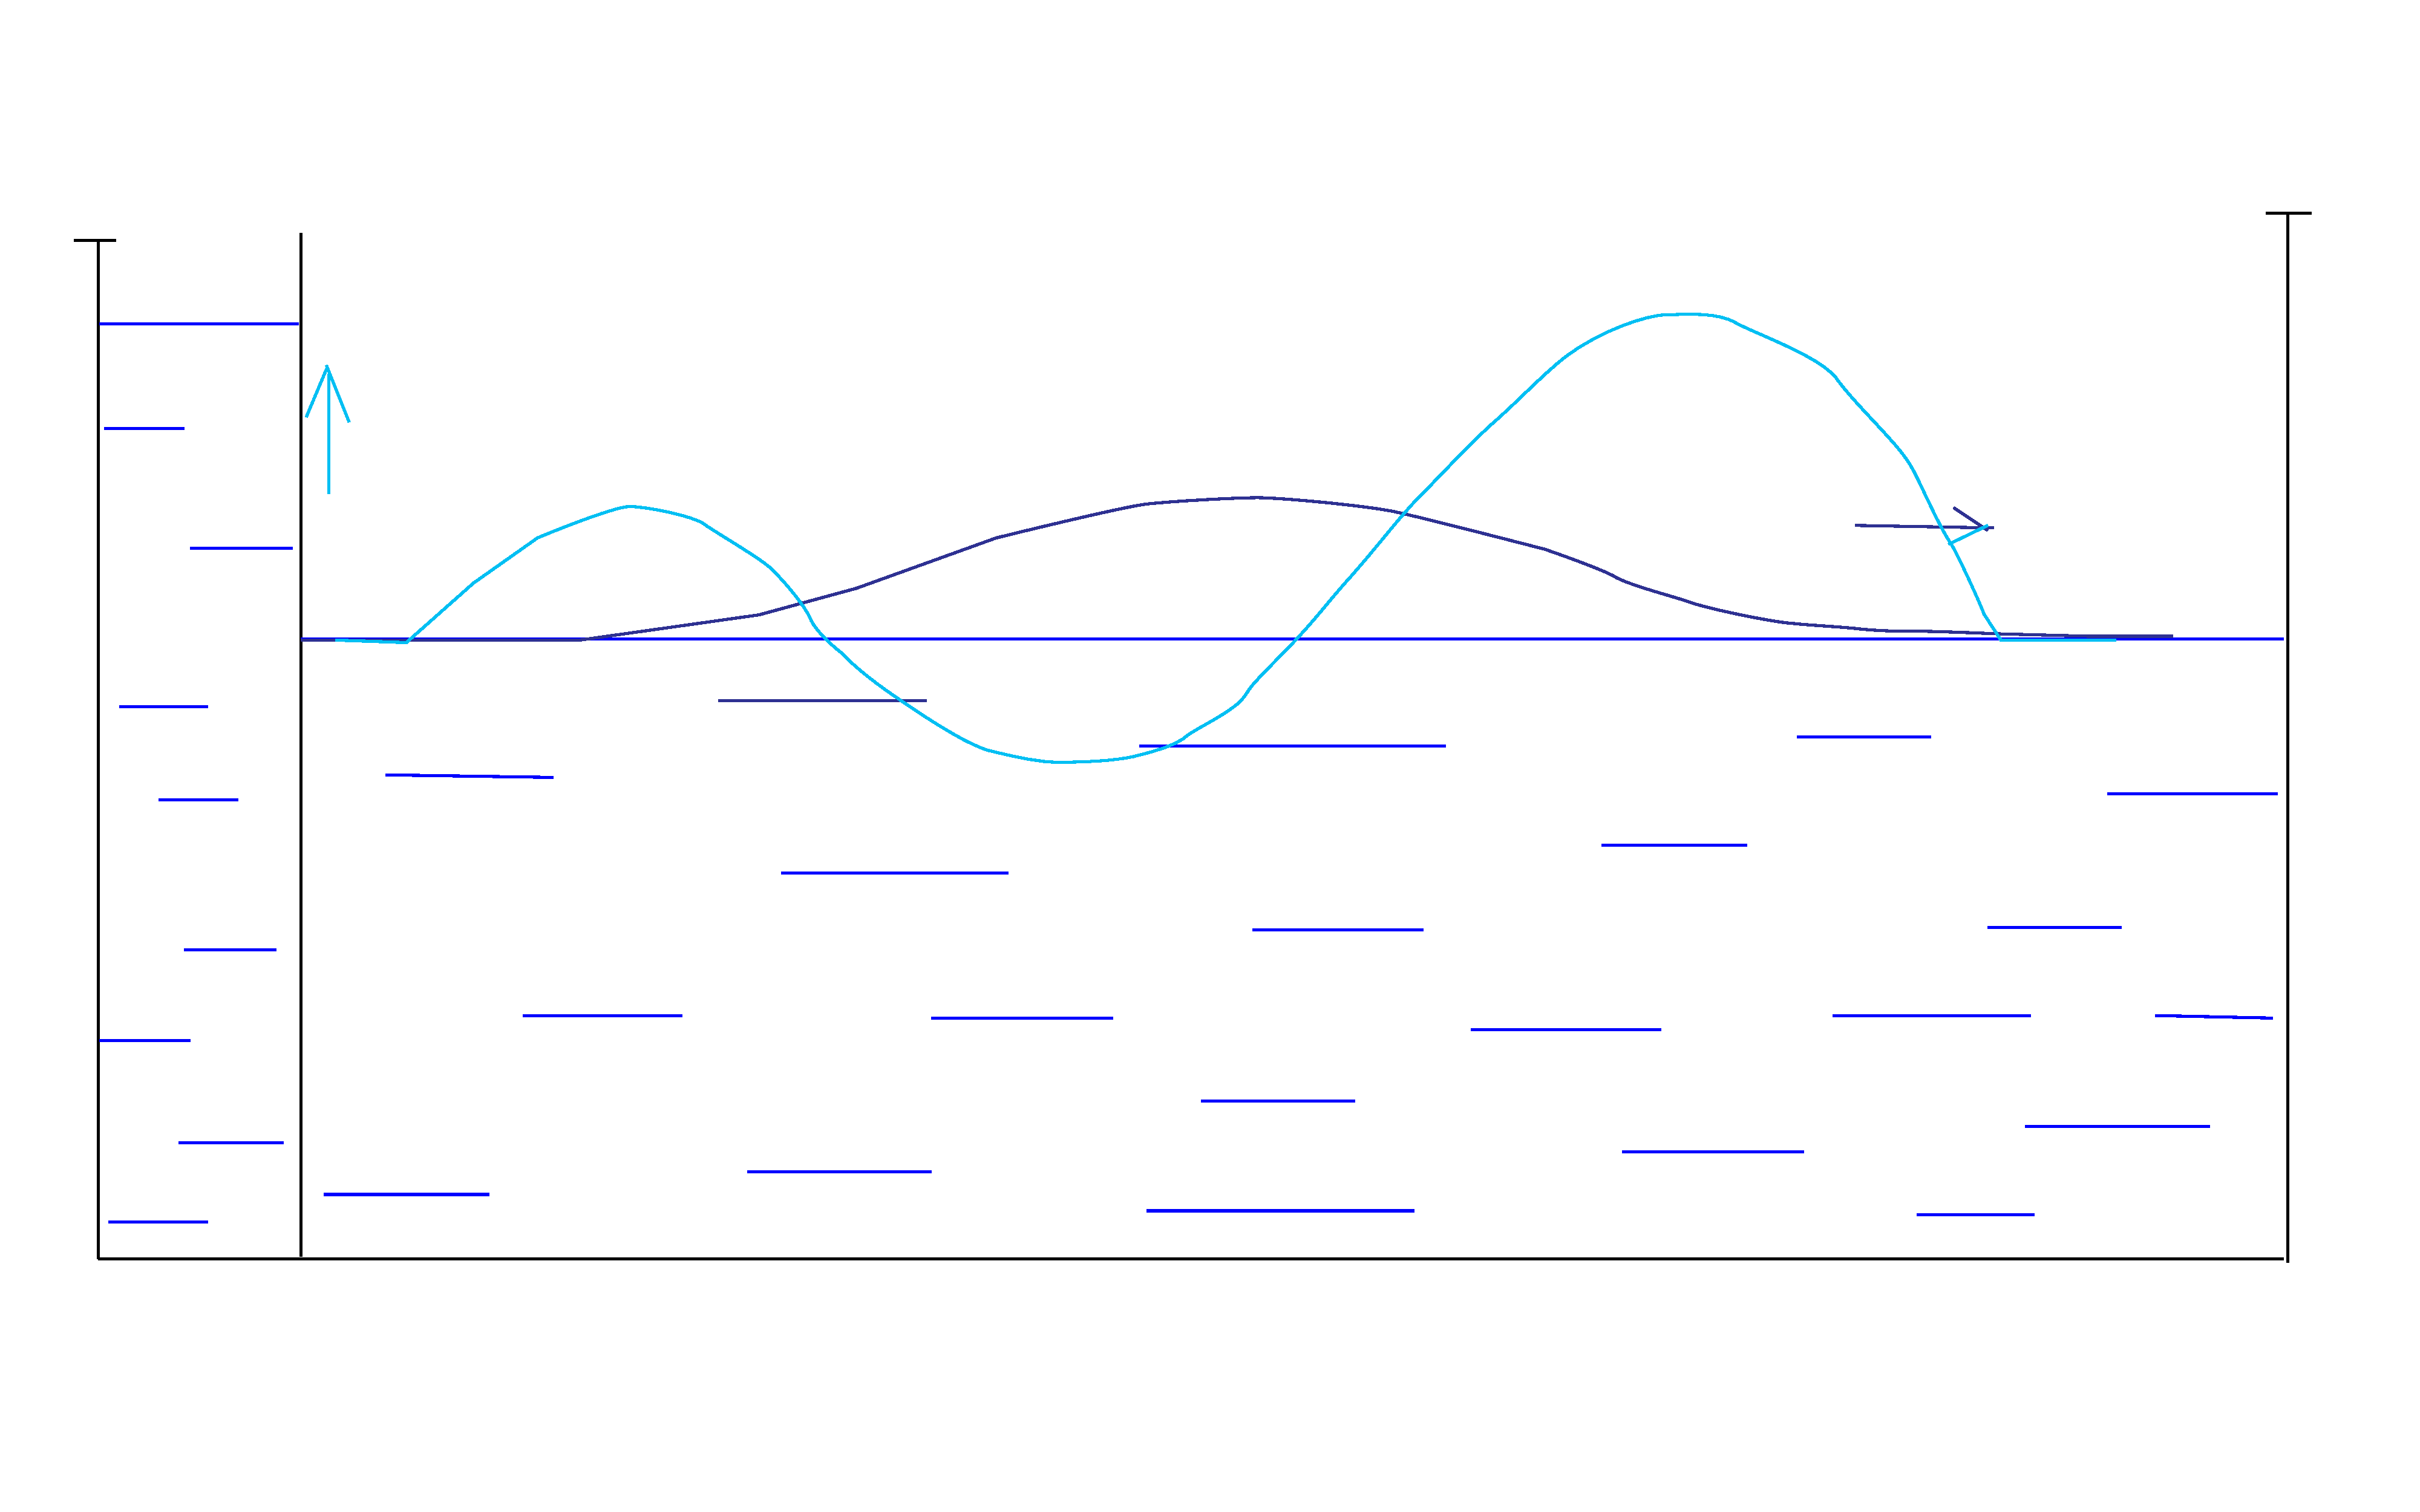
\includegraphics[width=0.4\linewidth]{fig/fig18.pdf}   
\end{figure}

Подбирают соотношение масс воды в емкостях. Резко поднимают задвижку. В зависимости от соотношения масс воды, могут побежать разные волны, разное количество холмов. 

Канал, который мы рассматриваем, мелкий, средней глубины $l$; $l+\eta(x,t)$. Поверим на слово: 
\begin{equation*}
	\pdv{\eta}{t}=\frac32 \sqrt{\frac{g}{l}}\pdv{}{x}\qty(\frac32 \alpha \eta+\frac12 \eta^2+\frac13 \sigma \pdv[2]{\eta}{x}),
\end{equation*}
где $\sigma=\frac{l^3}{3}-\frac{Tl}{\rho g}$, $\alpha$-произвольная константа, $T$ - коэффициент поверхностного натяжения, $\rho$ - плотность жидкости.

Преобразовав, получим
\begin{equation}
	\pdv{U}{t}+U\pdv{U}{x}+\beta \pdv[3]{U}{x}=0.
	\label{eq:33}
\end{equation}
$\beta$ - некоторая константа, а последнее слагаемое характеризует дисперсию. Видно, что уравнение простой волны дополняется дисперсией. (К экзамену построить дисперсионную характеристику). 

Пусть есть квадратичная среда, в нее запускают волну $e^{i(\omega_o t+kx)}$. Среда нелинейная и без дисперсии. При таких условиях квадратичная среда порождает новые частоты. $\omega_o$ порождает $2\omega_o$. Если нет дисперсии, то нет пространственных масштабов. $2\omega_o$ порождает $3\omega_o$ и так далее, лавинно. Спектр стремится в бесконечность. 
\begin{figure}[H]
	\centering
	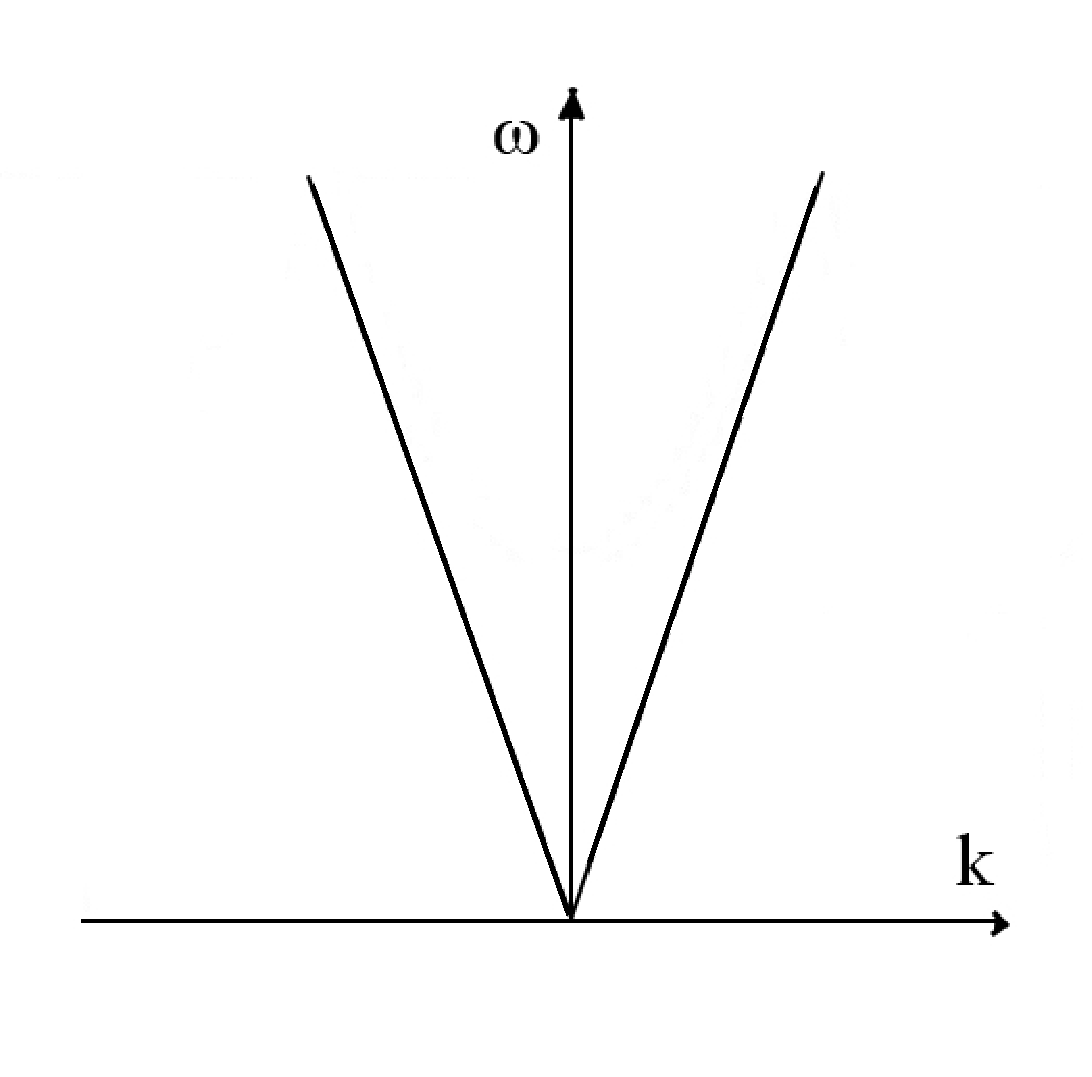
\includegraphics[width=0.4\linewidth]{fig/fig4.pdf}   
\end{figure}

Теперь включим дисперсию (в данном случае - высокочастотную). Она ограничивает частотный рост и стабилизирует волну. 

Будем искать решение уравнения \eqref{eq:33} в виде $U=U(x-Vt)$:
\begin{equation}
	-\pdv{U}{\xi}+U\pdv{U}{\xi}+\beta \pdv[3]{U}{\xi}=0.
	\label{eq:34}
\end{equation}

Интегрируя:
\begin{equation}
	\beta \pdv[2]{U}{\xi}+\frac{U^2}{2}-VU=0.
	\label{eq:35}
\end{equation}

Это есть уравнение нелинейного осциллятора. Для простоты константу интегрирования приравняли  к нулю, что дает уровень, откуда изменяется $U(x,t)$.
\begin{equation}
	\begin{cases}
		\dot{U}=y \\
		\beta \dot{y} =VU-\frac{U^2}{2}.		
	\end{cases}
	\label{eq:36}
\end{equation}

Получили систему для нелинейного осциллятора.
\begin{gather*}
	\beta \frac{y^2}{2}+E_{\text{п}} = const, \\ E_{\text{п}} = \frac{U^3}{6}-V\frac{U^2}{2}
\end{gather*}
\begin{figure}[H]
	\centering
	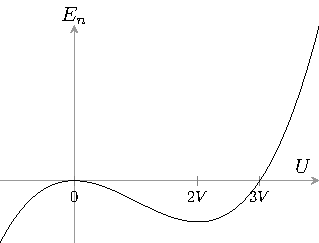
\includegraphics[width=0.4\linewidth]{fig/fig19.pdf}   
\end{figure}

Фазовый портрет:
\begin{figure}[H]
	\centering
	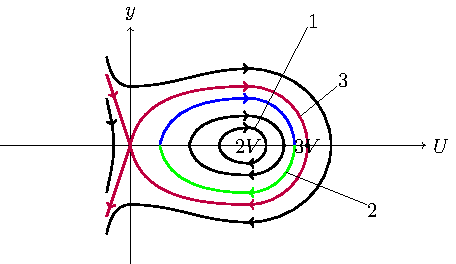
\includegraphics[width=0.5\linewidth]{fig/fig20.pdf}   
\end{figure}
Солитоном и является эта, покрашенная в восхитительный purple, гомоклиническая орбита.

22.04

Напомню, что дифференцирование в системе \eqref{eq:36} производится по бегущей координате. 

Вернемся к фазовому портрету. Неограниченные траектории лишены физического смысла, поэтому нас интересуют только ограниченные, то есть те, что находятся внутри петли сепаратрис, включая ее саму.

Пусть 1 - траектория вблизи состояния равновесия центр. Она замкнутая, колебание близко к гармоническому. Колебание происходит на фоне колебаний 2V. Таких колебаний континуум. 
\begin{figure}[H]
	\centering
	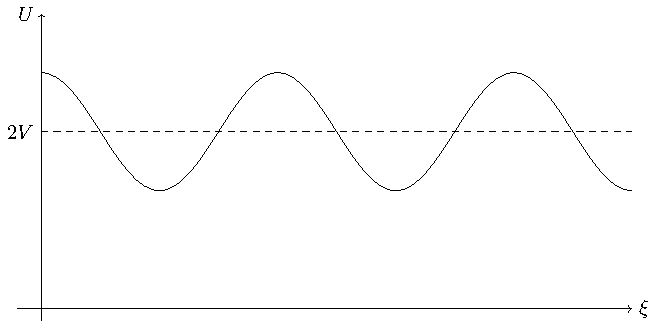
\includegraphics[width=0.4\linewidth]{fig/fig21.pdf}   
\end{figure}

Выберем 2 - вблизи седла, но все еще внутри гомоклинической орбиты. Выберем точку и положим при $\xi=0$ амплитуда максимальна. При движении по траектории к седлу (зеленым), U убывает. 
\begin{figure}[H]
	\centering
	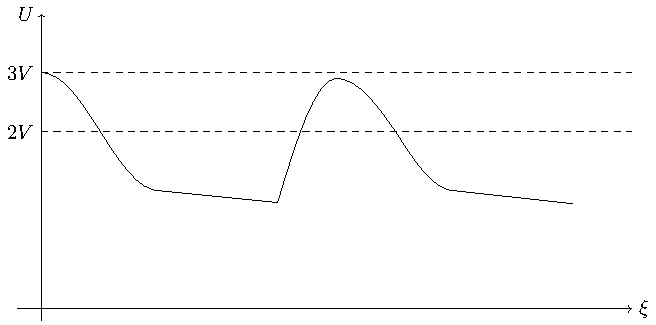
\includegraphics[width=0.4\linewidth]{fig/fig22.pdf}   
\end{figure}
Около самого состояния равновесия скорость мала, движение в ее окрестности будет проходить медленно. В конце концов, при выходе из окрестности состояния равновесия, скорость опять увеличится. Мы получим профиль, так называемой, кноидальной волны, которая далека от гармонической. Волны такие, потому что система нелинейная. 
Если брать траектории все ближе к седлу, полка будет увеличиваться. В конце концов, когда попадем на петлю:

Для того, чтобы нарисовать профиль в область $\xi<0$, нужно пройти по траектории в обратную сторону (синим). Рисунок качественный, нарисован из понимания поведения функции на концах и зная максимальную амплитуду. 
\begin{figure}[H]
	\centering
	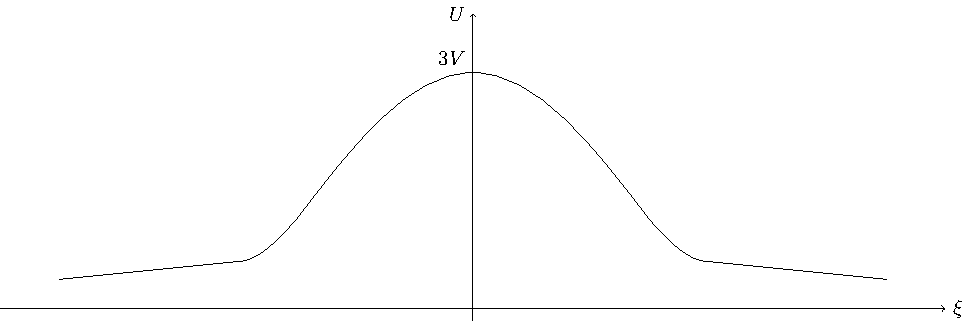
\includegraphics[width=0.4\linewidth]{fig/fig23.pdf}   
\end{figure}
Получившийся одиночный холм - это математический образ солитона. Точка 0 - решение, там нет пересечения траекторий, они стремятся туда асимптотически. 

Запишем наше уравнение в виде:

\begin{equation}
	\beta\dv[2]{U}{\xi}=VU-\frac{U^2}{2}
	\label{eq:37}
\end{equation}

Решение будем искать в виде:
\begin{equation}
	U=\frac{U_{max}}{\ch^2{(\xi / \Delta)}}
	\label{eq:38}
\end{equation}

Введенные параметры: $U_{max}, \Delta, V$ (V скрыто в $\xi=x-Vt$).
\begin{equation}
	\dv[2]{U}{\xi}=-2\frac{U_m}{\Delta^2}\frac{(3-2\ch^2{\xi / \Delta)}}{\ch^4{(\xi / \Delta)}}
	\label{eq:39}
\end{equation}
\begin{gather*}
	\frac{2\beta U_m}{\Delta^2}\frac{(3-2\ch^2{(\xi / \Delta))}}{\ch^4{(\xi / \Delta)}}=\frac{U_m V}{\ch^2{(\xi / \Delta)}}-\frac{U_m^2}{2\ch^4{(\xi / \Delta)}}.
\end{gather*}

Знаменатель не обращается в ноль.
\begin{gather*}
	-2\beta[3-2\ch^2{(\xi / \Delta)}]=\Delta^2 \ch^2{(\xi / \Delta)}V-\frac{U_m \Delta^2}{2}, \\
	-6\beta=\frac{U_m \Delta^2}{2}, \\
	4\beta=\Delta^2V.
\end{gather*}
\begin{equation}
	U_m \Delta^2= 12\beta,
	\label{eq:40}
\end{equation}
\begin{equation}
	\Delta^2V=4\beta.
	\label{eq:41}
\end{equation}
Параметры связаны, но их 3, а условия 2. Задав один, два других найдутся из \eqref{eq:40} и \eqref{eq:41}. $\beta$ характеризует дисперсию, не относится к самому солитону. V - скорость солитона, $U_m$ - его высота, $\Delta$ оказывается шириной. Ширина солитона вычисляется на уровне $U=\frac{4U_m}{2+e}$. 

Из уравнения \eqref{eq:41} следует, что, чем шире солитон, тем меньше его скорость: $V=\frac{4\beta}{\Delta^2}$. Из \eqref{eq:40}, что тогда и меньше амплитуда: $U_m=\frac{12\beta}{\Delta^2}$.

Если в диссипативной системе есть петля, то при изменении параметров она разрушается.Есть всего одна траектория, формирующая солитон. Солитоны устойчивы относительно большого числа начальных распределений. 

\subsection{Устойчивость солитона}
Замечание: рассмотрим уравнение Шредингера для определения статистического состояния. 
\begin{equation}
	\dv[2]{\psi}{x}+[U(x)+\epsilon]\psi=0.
	\label{eq:42}
\end{equation}

$U(x)>0, ~U\rightarrow 0$ при $x\rightarrow \pm \infty$

Есть решение, когда спектр дискретный: $\epsilon=\epsilon_n, \psi, \psi' \rightarrow 0$ при $x\rightarrow \pm \infty$.\

Существует связь между \eqref{eq:41} и устойчивостью солитонов уравнения Кортевега - де Фриза. Надо подставить нормированное решение:
\begin{equation*}
	\dv[2]{\psi}{x}+[\frac{1}{6\beta}U(x,t)+\epsilon]\psi=0.
\end{equation*}

Покажем, что, если речь о солитоне, то $\epsilon$ не будет зависеть от t.
\begin{equation*}
	U(x,t)=-6\beta(\frac{\psi''}{\psi}+\epsilon),
\end{equation*}
здесь $'$ - дифференцирование по x. Подставим в уравнение Кортевега - де Фриза:
\begin{equation*}
	\pdv{U}{t}+U\pdv{U}{x}+\beta \pdv[3]{U}{x}=0.
\end{equation*}
\begin{equation}
	\psi^2\dv{\epsilon}{t}=(\psi'A-A\psi').
	\label{eq:43}
\end{equation}
\begin{equation*}
	A(x,t)=6\beta(\frac1{\beta}\pdv{\psi}{t}-3\frac{\psi'\psi''}{\psi}+\psi'''-\frac{\epsilon}{6}\psi').
\end{equation*}

Проинтегрируем \eqref{eq:42} по переменной x в бесконечных пределах. Вспомним, что $\psi, \psi' \rightarrow 0$ при $x\rightarrow \pm \infty$. Получим:
\begin{equation*}
	\dv{\epsilon}{t}\int^{+\infty}_{-\infty}\psi^2dx=0.
\end{equation*}

В силу нормировки интеграл не равен нулю. Следовательно, $\dv{\epsilon}{t}=0$ и $\epsilon\neq \epsilon(t)$.
\begin{equation*}
	U(x,t)=U_{max}c\ch^{-2}(\frac{x-Vt}{\Delta}).
\end{equation*}

Здесь t можно выбрать любое. Положим, $t=0$.
\begin{equation}
	\psi''+(U_0 \ch^{-2}\alpha x+\epsilon)\psi=0.
	\label{eq:44}
\end{equation}
\begin{equation*}
	U_0=\frac{U_m}{6\beta},~\alpha=\frac1{\Delta}.
\end{equation*}

Пользуясь случаем, передаем приветы и спасибо третьему тому Ландау-Лившица, параграф 23, задача 4, где это уравнение решено. Спектр:
\begin{gather*}
	\epsilon_n=-\alpha(s-n), n=0,1,2,\dots;~n<s \\ s=\frac12(-1+\sqrt{1+\frac{4U_0}{\alpha^2}})=\frac12(-1+\sqrt{\frac{4U_m\Delta^2}{6\beta}})=\frac12(-1+3)=1 \\ \epsilon_n=-\alpha(1-n) \\ n=0:~ \epsilon_0=-\alpha^2=-\frac{4U_m}{12\beta}.
\end{gather*}

Если в уравнение Шредингера подставить уравнение солитона, такому потенциалу соответствует одно собственное значение. Пусть в начальный момент есть распределение (положительно определенное, но не совпадающее с солитоном). Подставляя его в уравнения Шредингера, решив, получим столько $\epsilon_j$, сколько солитонов может существовать при таких начальных условиях.
\begin{figure}[H]
	\centering
	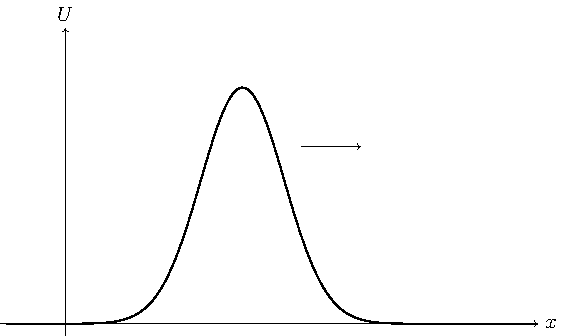
\includegraphics[width=0.4\linewidth]{fig/fig25.pdf}   
\end{figure}

Пусть $j=3$:
\begin{figure}[H]
	\centering
	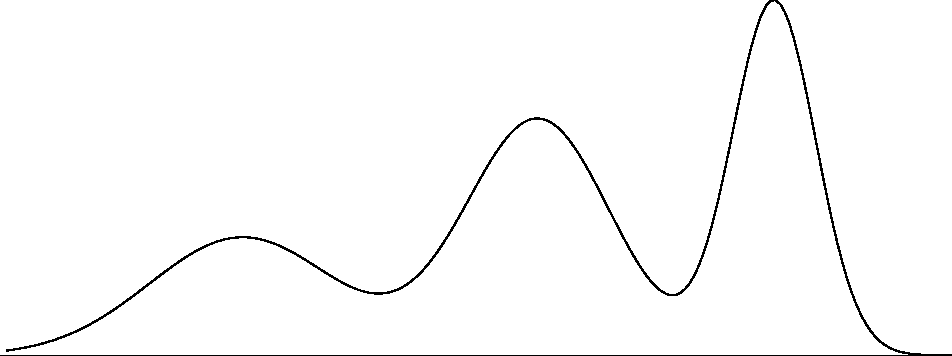
\includegraphics[width=0.4\linewidth]{fig/fig26.pdf}   
\end{figure}

Это обратная задача рассеяния. Качественные рассуждения: введем величину (из \eqref{eq:40}) $\sigma=\frac{\Delta^2 U_m}{12 \beta}=1$. Здесь $U_m$ характеризует нелинейность, а $\beta$ - дисперсию. Предположим, что при $t=0$ задали такое распределение, что $\sigma \ll 1$. Это означает малость $U_m$, мы находимся около стационарного состояния (около нуля). Если мы близки к линейной задаче, главную роль играют дисперсионные механизмы. Есть области прозрачности и непрозрачности. В области прозрачности фазовая скорость у каждой компоненты своя, пакет расплывается.  Приходим к единственному солитону.

Если  $\sigma \gg 1$, преобладает нелинейность. Она порождает новые гармоники. Переход к образованию состава из солитонов. Дисперсия ограничивает частоты, фронт стабилизируется.

\section{Стационарные ударные волны}
Рассмотрим
\begin{equation}
	\pdv{U}{t}+U\pdv{U}{x}+\beta \pdv[3]{U}{x}-\nu\pdv[2]{U}{x}=0.
	\label{eq:45}
\end{equation}

$\nu>0$ - диссипация. К чему приведет ее учет?

Если $\beta=0$, то уравнение называется уравнением Бюргерса. 

$\xi=x-Vt$ - называют стационарным решением, т.к. профиль не меняется. 
\begin{equation*}
	-V\dv{U}{\xi}+U\dv{U}{\xi}+\beta\dv[3]{U}{\xi}-\nu\dv[2]{U}{\xi}=0.
\end{equation*}

Проинтегрируем:
\begin{equation*}
	\beta\dv[2]{U}{\xi}-\nu \dv{U}{\xi}+\frac{U^2}{2}-VU=0.
\end{equation*}
($\cdot$ - дифференцирование по $\xi$)
\begin{equation}
	\begin{cases}
		\dot{U}=y \\
		\beta \dot{y} =\nu y-\frac{U^2}{2}+VU.		
	\end{cases}
	\label{eq:46}
\end{equation}

Система определена на фазовой плоскости. Состояния равновесия: $O_1(0,0)$, $O_2(2V,0)$. Линеаризуем в этих точках. $O_1$ - седло, а для $O_2$:
\begin{gather*}
	p^2-\frac{\nu}{\beta}p+\frac{V}{\beta}=0, \\ p_{1,2}=\frac{\nu}{2\beta}\pm \sqrt{\frac{\nu^2}{4\beta^2}-\frac{V}{\beta}}.
\end{gather*}

Если $\frac{\nu^2}{4\beta^2}-\frac{V}{\beta}<0$, то имеем неустойчивый фокус.
\begin{equation*}
	\frac{\nu^2}{4\beta}=V \rightarrow \beta=\frac{\nu^2}{4V}.
\end{equation*}
\begin{figure}[H]
	\centering
	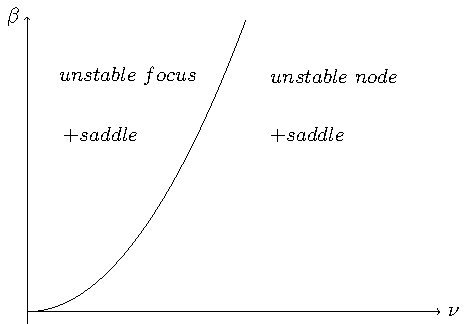
\includegraphics[width=0.4\linewidth]{fig/fig27.pdf}   
\end{figure}

Возьмем полную энергию при $\nu=0$:
\begin{equation*}
	V(U,y)=\beta\frac{y^2}{2}+\frac{U^3}{6}-V\frac{U^2}{2},
\end{equation*}

\begin{figure}[H]
	\centering
	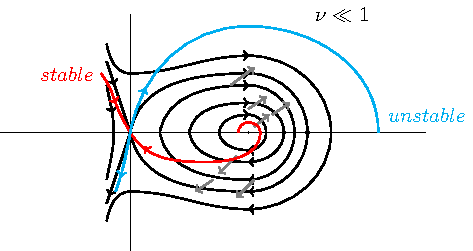
\includegraphics[width=0.4\linewidth]{fig/fig30.pdf}   
\end{figure}

\begin{equation*}
	\dot{V}=\beta y \dot{y}+\frac{U^2}{2}\dot{U}-VU\dot{U}=\nu y^2-\frac{U^2}{2}y+VUy-VUy+\frac{U^2}{2}y=\nu y^2\geqslant 0,
\end{equation*}
т.е. траектории системы пересекают линии уровня в сторону возрастания. Из существования этой функции следует, что система не имеет предельных циклов. 

Как ведут себя устойчивые сепаратрисы седла? Ограниченное решение существует, оно единственно и соответствует красной траектории. Зафиксируем $\beta$:
\begin{figure}[H]
	\centering
	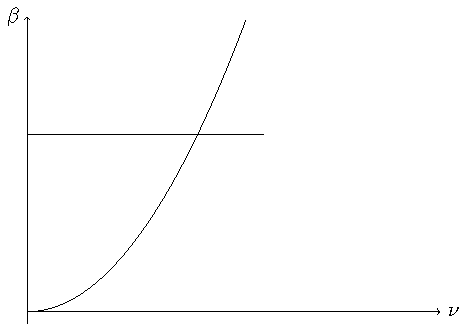
\includegraphics[width=0.4\linewidth]{fig/fig28.pdf}   
\end{figure}

Нарисуем профиль этой волны (для траектории, котора успеет сделать много витков, до того, как придет в состояние равновесия) ($\nu\ll1$):
\begin{figure}[H]
	\centering
	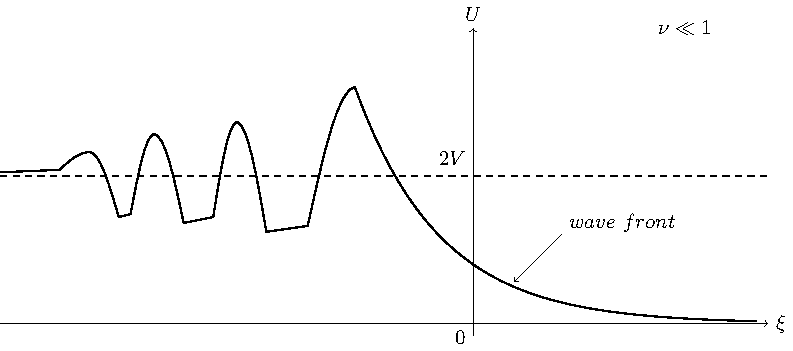
\includegraphics[width=0.6\linewidth]{fig/fig29.pdf}   
\end{figure}

Чем дальше от седла, тем ближе точки, выше и меньше полки. Это ударная волна.  Среда была в покое, прошел фронт и перебросил среду в новое состояние $2V$.

Для красной траектории:
\begin{figure}[H]
	\centering
	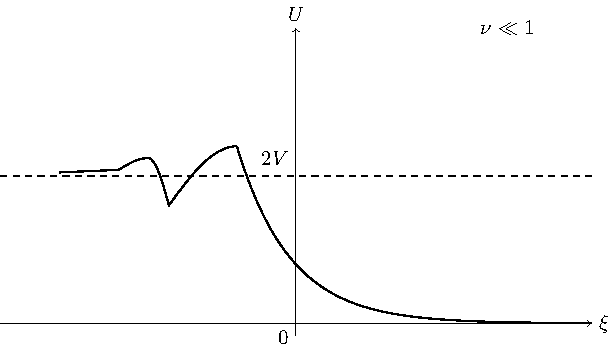
\includegraphics[width=0.6\linewidth]{fig/fig31.pdf}   
\end{figure}

Для траектории, идущей из неустойчивого состояния равновесия (фокуса или узла) в седло:
\begin{figure}[H]
	\centering
	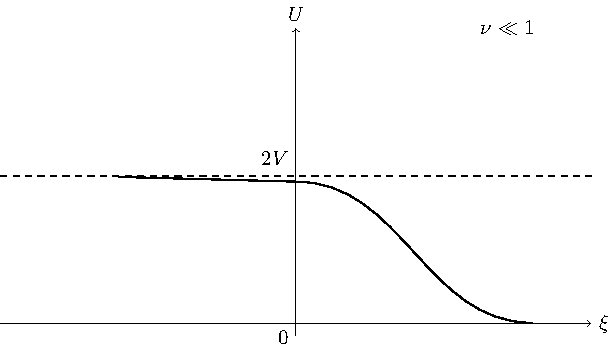
\includegraphics[width=0.6\linewidth]{fig/fig32.pdf}   
\end{figure}

Здесь не будет осцилляций. Во всех случаях есть передний фронт.

\section{29.04.19 Параметрические колебания}
Ранее мы рассматривали системы, в которых под действием внешних силовых воздействий появлялись новые режимы. Они являлись неавтономными. Кроме них существует другой тип неавтономных систем и внешнего воздействия. Внешнее воздействие находится внутри системы и может изменять его параметры. Они называются параметрическими, а колебания - параметрическими колебаниями. Пример - маятник, длина которого периодически меняется, т.е. параметр длины меняется со временем. 

Параметрические системы делят на 2 важных класса: резонансные и нерезонансные. В резонансных системах период изменения параметров находится в целочисленном соотношении с периодом собственных колебаний. В таких системах в такт с изменением энергии, соответствующей собственным колебаниям, вносится энергия, вызванная работой внешнего воздействия. При определенных условиях это может приводить к эффекту раскачки колебаний за счет накапливающейся в системе энергии. Этот эффект лежит в основе работы параметрических усилителей и генераторов. 

К нерезонансным неколебательным параметрическим системам относятся системы, в которых параметры изменяются очень быстро или очень медленно по сравнению с характерным временными масштабами изменения переменных системы. Динамика линейных параметрических систем описывается системой линейных дифференциальных уравнений с периодическими коэффициентами. 

Далее будем рассматривать только линейные параметрические системы. В основе теории таких систем лежит так называемая теория Флоке. 

Рассмотрим систему:
\begin{equation}
	\begin{cases}
		\dot{x_1}=p_{11}(t)x_1+p_{12}(t)x_2 \\
		\dot{x_2}=p_{21}(t)x_1+p_{22}(t)x_2.		
	\end{cases}
	\label{eq:47}
\end{equation}
\begin{equation*}
	p_{jk}(t+T)=p_{jk}(t),
\end{equation*}
т.е. коэффициенты периодически изменяются во времени. Запишем общее решение в матричном виде:
\begin{gather*}
	\vec{x} = X \vec{C}, \\
	\vec{x}= 
	\begin{pmatrix}
		x_1 \\
		x_2
	\end{pmatrix}
	,
	\vec{C}= 
	\begin{pmatrix}
		c_1 \\
		c_2
	\end{pmatrix}
	,
	\vec{X(t)}= 
	\begin{pmatrix}
		\phi_1 ~~  \psi_1 \\
		\phi_2  ~~ \psi_2
	\end{pmatrix}
	,
\end{gather*}
где векторы 
\begin{gather*}
	\vec{\phi}= 
	\begin{pmatrix}
		\phi_1 \\
		\phi_2
	\end{pmatrix}
	,
	\vec{\psi}= 
	\begin{pmatrix}
		\psi_1 \\
		\psi_2
	\end{pmatrix}
\end{gather*}
являются линейно не зависимыми, следовательно, образуют фундаментальную систему решений. 

Покажем, что в качестве таких функций можно выбрать такие функции, которые удовлетворяют начальным условиям:
\begin{gather}
	\phi_1(0)=1, \psi_1(0)=0, \notag \\ 
	\phi_2(0)=0, \psi_2(0)=1.		
	\label{eq:48}
\end{gather}

Согласно общей теории линейных дифференциальных уравнений вектора $\phi$, $\psi$  будут линейно не зависимы, если определитель Вронского не обращается в ноль:
\begin{gather*}
	W(t)= 
	\begin{vmatrix}
		\phi_1(t) ~~\psi_1(t) \\ 
		\phi_2(t) ~~\psi_2(t)
	\end{vmatrix}
	,
\end{gather*}
\begin{equation}
	W(t)=W(0)exp\qty[\int_0^t(p_{11}(t)+p_{22}(t))dt].
	\label{eq:49}	
\end{equation}

Для начальных условий \eqref{eq:48}: $W(0)=1$. отсюда следует, что вронскиан отличен от нуля, следовательно $\phi$, $\psi$ линейно не зависимы и образуют ФСР.

Поскольку $p_{jk}(t)$ являются периодическими, то вектора $\vec{\phi}(t+T)$, $\vec{\psi}(t+T)$ также линейно не зависимы и являются решением системы \eqref{eq:47}. Как всякое решение, эти вектора можно выразить через ФСР:
\begin{gather}
	\vec{\phi}(t+T)=a\vec{\phi}(t)+b\vec{\psi}(t) \notag \\ 
	\vec{\psi}(t+T)=c\vec{\phi}(t)+d\vec{\psi}(t),		
	\label{eq:50}
\end{gather}
где $a,b,c,d$ - некоторые константы. Можно переписать в скалярном виде, подставив $t=0$:
\begin{equation}
	a=\phi_1(T),~ b=\phi_2(T),~ c=\psi_1(T),~ d=\psi_2(T).
	\label{eq:51}	
\end{equation}

Соотношения \eqref{eq:51} говорят, что константы могут быть найдены, если известно общее решение.

Покажем, что для системы  \eqref{eq:47} справедливо:
\begin{equation}
	\vec{x}(t+T)=s\vec{x}(t),
	\label{eq:52}	
\end{equation}
т.е. через период решение повторяется с точностью до множителя.

Поскольку решение \eqref{eq:47} можно получить из общего, подобрав константы, то:
\begin{equation}
	\vec{x}(t)=A\vec{\phi}(t)+B\vec{\psi}(t),
	\label{eq:53}	
\end{equation}

Запишем состояние этого вектора в момент времени $t+T$:
\begin{equation}
	\vec{x}(t+T)=A\vec{\phi}(t+T)+B\vec{\psi}(t+T),
	\label{eq:54}	
\end{equation}

С другой стороны, подставим \eqref{eq:53} и \eqref{eq:54} в \eqref{eq:52}:
\begin{equation}
	A\vec{\phi}(t+T)+B\vec{\psi}(t+T)=s\qty[A\vec{\phi}(t)+B\vec{\psi}(t)].
	\label{eq:55}	
\end{equation}

Теперь используем \eqref{eq:50}:
\begin{equation}
	\qty[A(a-s)+Bc]\vec{\phi}(t)+\qty[Ab+B(d-s)]\vec{\psi}(t) \equiv 0.
	\label{eq:56}	
\end{equation}
Для выполнения равенства при любом t нужно, чтобы скобки с коэффициентами обратились в ноль.
\begin{equation}
	\begin{cases}
		A(a-s)+Bc=0 \\
		Ab+B(d-s)=0.		
	\end{cases}
	\label{eq:57}
\end{equation}

Это СЛОУ относительно коэффициентов A,B. Раскрываем определитель:
\begin{equation}
	s^2-(a+d)s+ad-bc=0.
	\label{eq:58}	
\end{equation}

Оказывается, что $ad-bc$ всегда можно найти, не находя общего решения.

Вернемся к вронскиану. Подсчитаем его в момент времени T:
\begin{gather*}
	W(T)= 
	\begin{vmatrix}
		\phi_1(T) ~~\psi_1(T) \\ 
		\phi_2(T) ~~\psi_2(T)
	\end{vmatrix}
	=
	\begin{vmatrix}
		a ~~c \\ 
		b ~~d
	\end{vmatrix}
	=ad-bc.
\end{gather*}
с другой стороны,
\begin{eqnarray*}
	W(T)=\underbrace{W(0)}_{\text{=1}}exp\qty[\int_0^T(p_{11}(t)+p_{22}(t))dt] \\
\end{eqnarray*}
\begin{equation}
	ad-bc=exp\qty[\int_0^T(p_{11}(t)+p_{22}(t))dt].
	\label{eq:59}
\end{equation}
$p_11, p_22$ знаем из постановки конкретной задачи.

Предположим, что \eqref{eq:58} не имеет кратных корней, следовательно, существует два значения мультипликатора и два решения:
\begin{gather}
	\vec{x_1}(t+T)=s_1\vec{x_1}(t) \notag \\ 
	\vec{x_2}(t+T)=s_2\vec{x_2}(t).		
	\label{eq:60}
\end{gather}

Таким образом, решение воспроизводит себя через период с точностью до множителя. 
\begin{gather}
	\vec{x_1}(t+nT)=(s_1)^n\vec{x_1}(t) \notag \\ 
	\vec{x_2}(t+nT)=(s_2)^n\vec{x_2}(t).		
	\label{eq:61}
\end{gather}

Покажем, что решения $\vec{x_1},\vec{x_2}$ можно представить в следующем виде:
\begin{gather}
	\vec{x_1}(t)=e^{\lambda_1t}\vec{\Phi_1}(t) \notag \\ 
	\vec{x_2}(t)=e^{\lambda_2t}\vec{\Phi_2}(t),		
	\label{eq:62}
\end{gather}
где $\lambda$ - некоторые числа, которые называются характеристическими. Функции имеют вид:
\begin{gather*}
	\vec{\Phi_1}(t)= 
	\begin{pmatrix}
		\Phi_{11} \\
		\Phi_{21}
	\end{pmatrix}
	,
	\vec{\Phi_2}(t)= 
	\begin{pmatrix}
		\Phi_{12} \\
		\Phi_{22}
	\end{pmatrix}
	,
\end{gather*}
и являются периодическими с периодом T:
\begin{equation}
	\Phi_{jk}(t+T)=\Phi_{jk}(t),
	\label{eq:63}
\end{equation}
а характеристические числа удовлетворяют:
\begin{gather}
	\lambda_j=\frac{1}{T}Ln(s_j)=\frac1{T}\qty[ln|s_j|\pm i(arg(s_j)+2\pi k)], \notag \\
	j=1,2;~~k=0,\pm 1, \pm 2, \dots.
	\label{eq:64}
\end{gather}
s-мультипликаторы, которые могут быть комплексными, поэтому присутствует аргумент комплексного числа.

Покажем справедливость \eqref{eq:63}. Из \eqref{eq:62}:
\begin{gather*}
	\vec{\Phi}_j(t)=e^{-\lambda_j t}\vec{x}_j(t), \\
	\vec{x}_j(t+T)=s\vec{x}_j(t)=e^{\lambda_0 T}\vec{x}_j(t), \\
	\vec{\Phi}_j(t+T)=e^{-\lambda_0(t+T)}\vec{x}_j(t+T)=e^{\lambda_0 T}\vec{x}_j(t)e^{-\lambda_j(t+T)}=\vec{x}_j(t)e^{-\lambda_j t}=\vec{\Phi}_0(t).
\end{gather*}

Можно записать:
\begin{equation}
	\vec{x}_j(t)=\sum_{j=1}^2 c_j e^{\lambda_j t}\vec{\Phi}_j(t).
	\label{eq:65}
\end{equation}

Это основное соотношение ЛДУ с переменными параметрами. Здесь $\Phi$ - функции Флоке. 

Замечание: теория Флоке может быть применена к предельным циклам, т.к. они есть переодическое решение. 
\subsection{Отображение через период}
С точки зрения теории динамических систем, \eqref{eq:47} - неавтономная система, следовательно, порождает точечное отображение $g^t:\mathds{R}^2\rightarrow \mathds{R}^2$.
\begin{figure}[H]
	\centering
	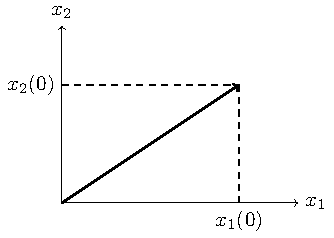
\includegraphics[width=0.35\linewidth]{fig/fig33.pdf}   
\end{figure}

Под действием системы \eqref{eq:47} вектор $\vec{x}(0)$ в некоторый момент времени t переходит в $\vec{V}(t)$
\begin{equation*}
	g^t\vec{x}(0)=\vec{V}(t).
\end{equation*}
если $t=0: \vec{x}(0)=\vec{V}(0)$.

В сиду теории Флоке наибольший интерес представляет отображение через период, т.е. $g^T$. Заметим, что решение $x_1=0, x_2=0$ является неподвижной точкой этого отображения. Более того, с точки зрения неавтономной системы, это периодическое решение любого периода. 

Воспользуемся соотношением Флоке:
\begin{gather}
	x_1(t)=C_1 e^{\lambda_1 t}\Phi_{11}(t)+C_2 e^{\lambda_2 t}\Phi_{12}(t) \notag \\ 
	x_2(t)=C_1 e^{\lambda_1 t}\Phi_{21}(t)+C_2 e^{\lambda_2 t}\Phi_{22}(t),		
	\label{eq:66}
\end{gather}
\begin{gather*}
	x_1=x_1(0), \\ 
	x_2=x_2(0),		
\end{gather*}
подставляем $t=0$ в \eqref{eq:66}, находим $C_1^0, C_2^0$ относительно них будет СЛНУ. Задаем точку, находим ее образ через период:
\begin{gather}
	x_1(t)=C_1^0 e^{\lambda_1 t}\Phi_{11}(t)+C_2^0 e^{\lambda_2 t}\Phi_{12}(t) \notag \\ 
	x_2(t)=C_1^0 e^{\lambda_1 t}\Phi_{21}(t)+C_2^0 e^{\lambda_2 t}\Phi_{22}(t),		
	\label{eq:67}
\end{gather}

Используя \eqref{eq:53}, а также связь A и B с a, b, c, d:
\begin{gather*}
	\Phi_{11}(0)=A_1,~\Phi_{12}(0)=A_2,~\Phi_{21}(0)=B_1,~\Phi_{22}(0)=A_2.	
\end{gather*}
\begin{equation}
	g^T\rightarrow
	\begin{cases}
		x_1(T)=a x_1(0)+c x_2(0) \\
		x_2(T)=b x_1(0)+d x_2(0)		
	\end{cases}
	\label{eq:68}
\end{equation}
\begin{gather*}
	\vec{x}(T)=G \vec{X}(0),~ G=
	\begin{pmatrix}
		a ~b \\
		c ~d \\
	\end{pmatrix}
	,\\
	a=\phi_1(T), ~ b=\phi_2(T), \\
	c=\psi_1(T), ~ d=\psi_2(T).
\end{gather*}

Траектории системы порождают порождают точечное отображение. Роль дискрета играет период T. Отображение линейное. Нужно исследовать устойчивость неподвижных точек. 
\subsection{Устойчивость нулевого решения}
Вспомним точечное отображение. Поведение $g^T$ зависит от мультипликаторов.

Пусть $s_1, s_2$ - действительные. Тогда \eqref{eq:68} с помощью преобразования можно привести к виду:
\begin{equation*}
	\begin{cases}
		U_1(T)=s_1 U_1(0) \\
		U_2(T)=s_2 U_2(0)		
	\end{cases}
\end{equation*}
\begin{enumerate} 
	\item Поскольку мультипликаторы $s_1, s_2$ соответствуют решениям неавтономной \eqref{eq:47} системы, они удовлетворяют условию $s_1\cdot s_2>0$;
	\item Если $|s_j|<1$, неподвижная точка устойчива, если $|s_j|>1$ - неустойчива. Если $|s_i|<1, |s_j|>1, s_i \neq s_j$, то точка - седло. 
\end{enumerate} 

Пусть $0<s_j<1$:
\begin{figure}[H]
	\centering
	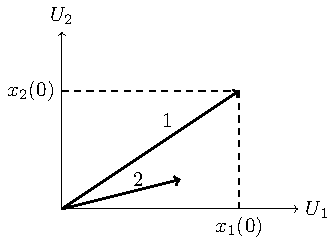
\includegraphics[width=0.35\linewidth]{fig/fig34.pdf}   
\end{figure}

Вектор уменьшит длину и повернется. Любое начальное условие стремится к нулю, следовательно, решение устойчивое.

$-1<s_j<0$:
\begin{figure}[H]
	\centering
	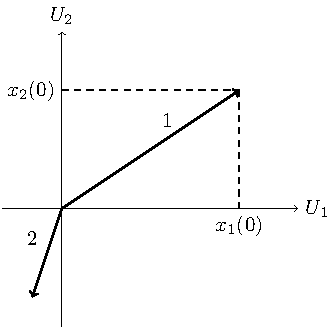
\includegraphics[width=0.35\linewidth]{fig/fig35.pdf}   
\end{figure}

Вектор уменьшит длину и переместится в отрицательную область. Будут скачки. Решение устойчиво.

$0<|s_1|<1, |s_2|>1$:
\begin{figure}[H]
	\centering
	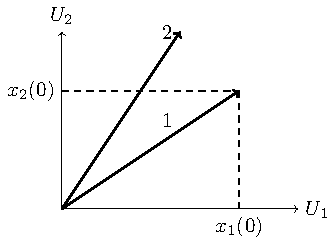
\includegraphics[width=0.35\linewidth]{fig/fig36.pdf}   
\end{figure}

По одной координате растяжение, а по другой сжатие. Вектор асимптотически прижимается к оси ординат.

$-1<|s_1|<0, |s_2|<-1$:
\begin{figure}[H]
	\centering
	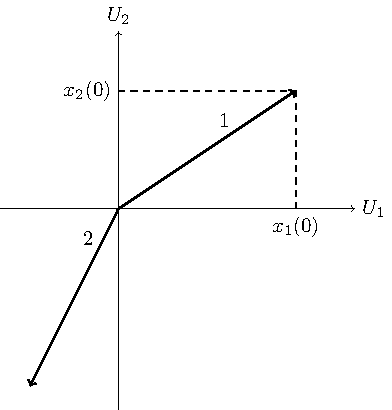
\includegraphics[width=0.35\linewidth]{fig/fig37.pdf}   
\end{figure}

Вектор прижимается к оси координат и растягивается.

29.04

Рассмотрим комплексно-сопряженные корни. Линейным преобразованием систему можно привести к нормальной форме.
\begin{equation}
	U_j(T)=s_j U_j(0), ~j=1,2.
	\label{eq:69}
\end{equation}

$|s|<1$ - длина вектора меняется.
\begin{equation}
	s_j=\alpha \pm i\beta.
	\label{eq:70}
\end{equation}
Поскольку мультипликаторы являются комплексно сопряженными, переменные $U_j(T), U_j(0)$ являются комплексными функциями. 
\begin{gather}
	U_j(0)=U(0)\pm iV(0) \notag \\ 
	U_j(T)=U(T)\pm iV(T).		
	\label{eq:71}
\end{gather}

Подставляя \eqref{eq:70}, \eqref{eq:71} в \eqref{eq:69} и разделяя реальную и мнимую части, получим:
\begin{gather}
	U(T)=\alpha U(0)- \beta V(0) \notag \\ 
	V(T)=\beta U(0)+ \alpha V(0).		
	\label{eq:72}
\end{gather}
\begin{gather*}
	U=\rho \cos{\phi}, V=\rho \sin{\phi}, \\ 
	s=\alpha \pm i\beta=|s|e^{\pm i \omega}, \\
	|s|=\sqrt{\alpha^2+\beta^2},		
\end{gather*}
\begin{gather}
	\alpha=|s|\cos{\omega} \notag \\ 
	\beta=|s|\sin{\omega}.		
	\label{eq:73}
\end{gather}
\begin{equation}
	\begin{cases}
		\rho(T)\cos{\phi(T)}=\alpha \rho(0)\cos{\phi(0)}-\beta \rho(0)\sin{\phi(0)} \\
		\rho(T)\sin{\phi(T)}=\beta \rho(0)\cos{\phi(0)}+\alpha \rho(0)\sin{\phi(0)}.
	\end{cases}
	\label{eq:74}
\end{equation}
Из этой системы находят $\rho(T)$ и $\phi(T)$:
\begin{equation}
	\begin{cases}
		\phi(T)=\phi(0)+\omega \\
		\rho(T)=|s|\rho(0).
	\end{cases}
	\label{eq:75}
\end{equation}

Эта система задает отображение $g^T$. Полярный угол $\phi$ меняется за период на $\omega$, а начальная величина вектора $\rho(0)$ изменяется в зависимости от s. 

Если $|s|<1$:
\begin{figure}[H]
	\centering
	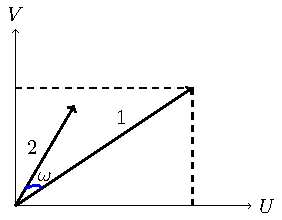
\includegraphics[width=0.35\linewidth]{fig/fig38.pdf}   
\end{figure}

Вектор поворачивается на угол $\omega$ и сокращается в длину. Состояние равновесия и соответствующая ему неподвижная точка $x_1=x_2=0$ являются асимптотически устойчивыми.

$|s|>1$:
\begin{figure}[H]
	\centering
	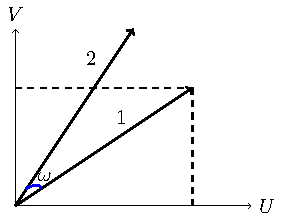
\includegraphics[width=0.35\linewidth]{fig/fig39.pdf}   
\end{figure}

Состояние равновесия неустойчивое, вектор поворачивается и растягивается.

$|s|=1$:
\begin{figure}[H]
	\centering
	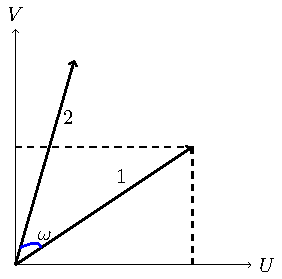
\includegraphics[width=0.35\linewidth]{fig/fig40.pdf}   
\end{figure}

Вектор поворачивается, длина его не меняется. 

Вектор, пройдя период, может либо совпасть с начальным, либо нет. В зависимости от этого решение будет периодическим или квазипериодическим.

Таким образом, состояние равновесия или периодическая траектория любого периода в параметрической системе может быть устойчивой либо не устойчивой.

\subsection{Основные режимы линейной параметрической системы}

Поскольку система линейная, из условия устойчивости состояния равновесия вытекают все остальные свойства линейных параметрических систем, а именно:
\begin{enumerate} 
	\item Параметрическая система, находящаяся в начальный момент в состоянии равновесия, останется в этом состоянии при $\forall t>0$, поскольку состояние равновесия $x_1=x_2=0$ существует всегда в линейной системе. Параметрическую систему, находящуюся в состоянии равновесия, нельзя вывести из этого состояния, изменяя ее параметры. Пример - маятник на нитке: дергая за нитку, маятник нельзя раскачать;
	\item Состояние равновесия параметрической системы может быть как устойчивым, так и не устойчивым;
	\item Если параметры системы таковы, что она неустойчива и система выведена из состояния равновесия, то в ней возникают колебания, амплитуда которых экспоненциально возрастает. Этот процесс возрастания размахов колебаний при периодическом нарастании колебаний, называется параметрическим резонансом.
\end{enumerate} 

\subsection{Параметрические колебания. Резонанс.}
Установим условие существования параметрического резонанса в одном частном, но важном случае. Рассмотрим систему \eqref{eq:47} в случае $p_{11}(t) \equiv0, p_{12}(t)\equiv 1, p_{22}(t) \equiv 0$, тогда система примет вид:
\begin{equation}
	\begin{cases}
		\dot{x_1}=x_2 \\
		\dot{x_2}=p_{21}(t)x_1.
	\end{cases}
	\label{eq:76}
\end{equation}

Система \eqref{eq:76} охватывает уравнения Матье и Хилла. 

Поведение системы определяют мультипликаторы, а они, в свою очередь, определяются характеристическим уравнением:
\begin{gather*}
	s^2-(a+d)s+(ad-bc)=0, \\
	ad-bc=exp\qty[\int_0^T(p_{11}(t)+p_{22}(t))dt]=1.		
\end{gather*}

Фактически, варьируются только коэффициенты a и d. Введем: $2P=a+d$ - контрольный параметр.
\begin{gather*}
	s^2-2Ps+1=0.		
\end{gather*}

Проанализируем поведение s.
Пусть $|P|<1$
\begin{gather*}
	s_{1,2}=P\pm i\sqrt{1-P^2}, \\
	|s|=1.		
\end{gather*}

Неподвижная точка отображения $g^T$ будет эллиптической. 

Достаточно рассмотреть только $x_1(t)$:
\begin{equation}
	x_1(t)=c_1e^{\lambda_1 t}\Phi_{11}(t)+c_2e^{\lambda_2 t}\Phi_{12}(t).
	\label{eq:77}
\end{equation}

Поскольку $|s|=1$, характеристические показатели $\lambda$ связаны с s: $\lambda_1=\frac{q}{T}i,~\lambda_2=-\frac{q}{T}i$, где $q=|arg(s_j)+2\pi k|$ (из формулы \eqref{eq:64}). $\lambda$ чисто мнимые, x действительные, следовательно, $c_1, c_2, \Phi_{11}, \Phi_{12}$ должны быть комплексными:
\begin{equation}
	\begin{cases}
		c_1=\frac{A}{2}e^{ic} \\
		c_2=\frac{A}{2}e^{-ic} \\
		\Phi_{11}=h(t)e^{i\varkappa(t)} \\
		\Phi_{12}=h(t)e^{-i\varkappa(t)}.
	\end{cases}
	\label{eq:78}
\end{equation}

Подставляя \eqref{eq:78} в \eqref{eq:77}, получим:
\begin{equation}
	x_1(t)=Ah(t)\cos (\frac{q}{T}t+c+\varkappa(t)).
	\label{eq:79}
\end{equation}

Вспомним косинус суммы, чтобы выделить соответственные временные масштабы. $h(t)$ и $\varkappa(t)$ периодичны с периодом T (из теории Флоке). T - период изменения параметров.
\begin{equation}
	x_1(t)=H(t)\cos{(\frac{q}{T}t+c)}+F(t)\sin{(\frac{q}{T}t+c)}.
	\label{eq:80}
\end{equation}
\begin{gather*}
	H(t)=Ah(t)\cos \varkappa(t), \\
	F(t)=-Ah(t)\sin \varkappa(t).		
\end{gather*}

В \eqref{eq:80} $H(t)$ и $F(t)$ периодичны с периодом T. Есть два временных масштаба: $T_1=T$ и $T_2=\frac{2\pi}{q}T$, которым отвечают частоты $\omega_1$ и $\omega_2$ соответственно.

$\frac{\omega_1}{\omega_2}=\frac{2\pi}{q}$, откуда вытекает, что, если $\frac{2\pi}{q}$ - рациональное число, то $x_1(t)$ - периодическая функция, если иррациональное, то $x_1(t)$ - квазипериодическая функция. Таким образом, при выполнении $P>1$, в системе \eqref{eq:76} реализуются ограниченные колебания, которые называются параметрическими.

Пусть $|P|>1$.

Из характеристического уравнения $s_1 \cdot s_2=1$, они действительны. Для определенности $|s_1|>1,~ |s_2|<1$.

Пусть $P>1$. Действует отображение $g^T$:
\begin{figure}[H]
	\centering
	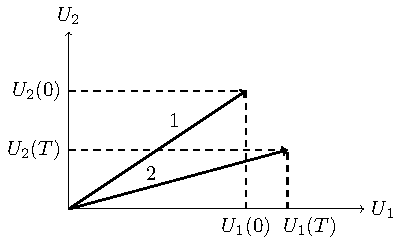
\includegraphics[width=0.35\linewidth]{fig/fig41.pdf}   
\end{figure}

По переменной $U_1$ увеличение вектора, по $U_2$ - уменьшение. Процесс повторяется. Вектор вытягивается и прижимается к оси абсцисс. Если $n\rightarrow \infty$ (число итераций): $U_2(nT)\rightarrow 0,~U_1(nT)\rightarrow \infty$. В системе реализуется параметрический параметрический резонанс. 

Получим приближенное соотношение для $x_1(t)$:
\begin{gather*}
	\lambda_1=\frac{1}{T}ln(s_1)>0, \\
	\lambda_2=\frac{1}{T}ln(s_2)=\frac{1}{T}ln(\frac{1}{s_1})=-\frac{1}{T}ln(s_1)<0.
\end{gather*}

Функция Флоке ограниченная
\begin{equation*}
	x_1(t)\approx c_1 e^{\frac{1}{T}ln(s_1)t}\Phi_{11}(t).
\end{equation*}
\begin{figure}[H]
	\centering
	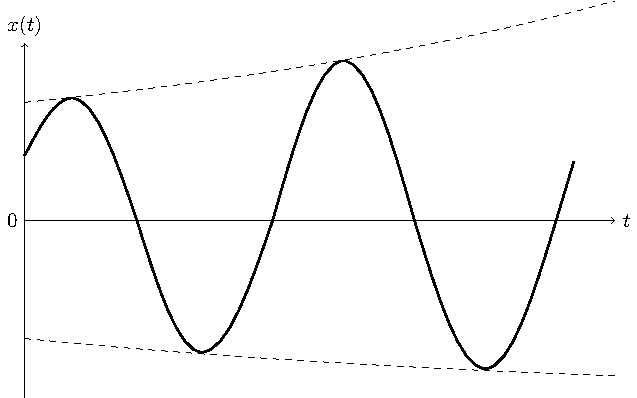
\includegraphics[width=0.5\linewidth]{fig/fig42.pdf}   
\end{figure}

В начальный момент система должна быть выведена из равновесия. Это геометрическая прогрессия, экстремумы функции лежат на экспоненте. 
\begin{itemize}
	\item В линейном осцилляторе экстремумы на прямых;
	\item Если линейный осциллятор в покое, мы можем его раскачать;
\end{itemize}

Пусть $s_1,s_2<0,~|s_1|>1,~|s_2|<1$:
\begin{figure}[H]
	\centering
	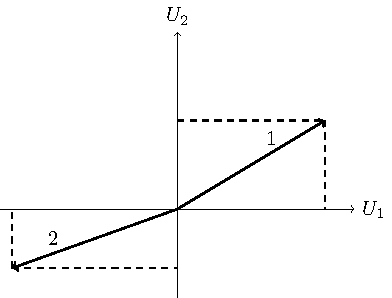
\includegraphics[width=0.5\linewidth]{fig/fig43.pdf}   
\end{figure}

Вектор вернется через 2 итерации, период 2T, экстремумы отстоят на период.
\begin{figure}[H]
	\centering
	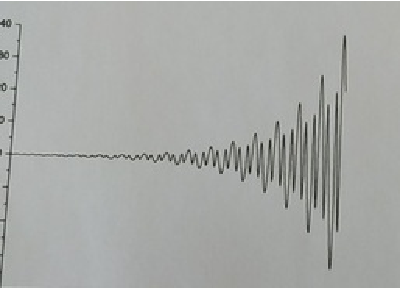
\includegraphics[width=0.4\linewidth]{fig/fig44.pdf}   
\end{figure}

Пусть $|P|=1$. В этом случае, если $P=1$, то $s_1=s_2=1$; если $P=-1$, то $s_1=s_2=-1$. Корни кратные, мы такое не рассматривали. Решение в этом случае задается в виде:
\begin{gather*}
	x_1(t)=c_1 e^{\lambda t}\Phi(t)+c_2te^{\lambda t}\Phi(t), \\
	\lambda=\frac{1}{T}ln|s|.
\end{gather*}

На границе неустойчивость и состояние равновесия $x_1=x_2=0$ является неустойчивым.

\subsection{Параметрические колебания маятника}
\begin{equation}
	\ddot{\varphi}+2\delta \dot{\varphi}+\frac{g}{l(t)}\varphi=0.
	\label{eq:81}
\end{equation}

Рассмотрим маятник, у которого длина периодически меняется, $\delta$ характеризует диссипацию. Кусочно-линейная аппроксимация. $l(t+T)=l(t)$.

Будем считать, длина меняется мгновенно:
\begin{equation*}
	l(t)=
	\begin{cases}
		l_0-\frac{a}{2}, 0 \leq t \leq \frac{T}{2} \\
		l_0+\frac{a}{2}, \frac{T}{2} \leq t \leq T		
	\end{cases}
\end{equation*}

далее периодично. Получается меандр.
\begin{equation*}
	l_0=\frac{a}{2}>0,~\omega_1^2=\frac{g}{l_0-\frac{a}{2}},~\omega_2^2=\frac{g}{l_0+\frac{a}{2}}.
\end{equation*}

Рассмотрим консервативный случай ($\delta=0$). Перепишем \eqref{eq:81} в виде:
\begin{equation}
	\begin{cases}
		\dot{\varphi}=y \\
		\dot{y} =-\omega^2(t)\varphi.	
	\end{cases}
	\label{eq:82}
\end{equation}
\begin{equation}
	\omega^2(t)=
	\begin{cases}
		\omega^2_1, 0 \leq t \leq \frac{T}{2} \\
		\omega^2_2, \frac{T}{2} \leq t \leq T		
	\end{cases}
	\label{eq:83}	
\end{equation}

\eqref{eq:82} является частным случаем рассмотренного выше, где $p_{21}=\omega^2(t)$. Для построения областей надо построить границы $P=\pm 1$, найдя a,d. Они являются элементами матрицы G. которая задает $g^T$. Поскольку система является кусочно-линейной, можно представить: $G=G_1\cdot G_2$, где $G_1$ действует на интервале от 0 до $\frac{T}{2}$, $G_2$ от $\frac{T}{2}$ до $T$. 

\underline{Матрица $G_1$:}

$\omega^2(t)\equiv\omega_1^2$

Решая \eqref{eq:82}:
\begin{gather*}
	\varphi_1(t)\equiv A_1 \cos(\omega_1 t) + B_1\sin(\omega_1 t), \\
	\varphi_2(t)\equiv -A_1 \sin(\omega_1 t) + \omega_1 B_1\cos(\omega_1 t).
\end{gather*}

Положим: $\varphi_1(0)=1,~\varphi_2(0)=0$. $A_1=1,~B_1=0$. Искомое решение примет вид: 
\begin{equation}
	\begin{cases}
		\varphi_1(t) = \cos(\omega_1 t) \\
		\varphi_2(t) = -\sin(\omega_1 t).		
	\end{cases}
	\label{eq:84}	
\end{equation}

Аналогично находится второе решение:
\begin{gather}
	\psi_1(0)=0, \psi_2(0)=1, \notag \\
	\begin{cases}
		\psi_1(t) = \frac{\sin(\omega_1 t)}{\omega_1} \\
		\psi_2(t) = \cos(\omega_1 t).		
	\end{cases}
	\label{eq:85}	
\end{gather}

Подставляя $t=\frac{T}{2}$, найдем элементы $G_1$:
\begin{equation}
	\begin{cases}
		a_1 = \cos(\omega_1 \frac{T}{2}) \\
		b_1 = -\omega_1 \sin(\omega_1 \frac{T}{2}) \\
		c_1 = \frac{\sin(\omega_1 \frac{T}{2})}{\omega_1} \\
		d_1 = \cos(\omega_1 \frac{T}{2}),	
	\end{cases}
	\label{eq:86}	
\end{equation}
\begin{gather*}
	G_1= 
	\begin{pmatrix}
		\cos \alpha~~~~~\frac{\sin\alpha}{\omega_1} \\
		-\omega_1 \sin \alpha~~\cos \alpha
	\end{pmatrix}
	, 
	\alpha=\omega_1 \frac{T}{2}.	
\end{gather*}

\underline{Матрица $G_2$:}
Вид устанавливается аналогично:
\begin{gather*}
	G_1= 
	\begin{pmatrix}
		\cos \beta~~~~~\frac{\sin\beta}{\omega_2} \\
		-\omega_2 \sin \beta~~\cos \beta
	\end{pmatrix}
	, 
	\beta=\omega_2 \frac{T}{2}.	
\end{gather*}

\underline{ $G_1\cdot G_2$:}

Получили матрицу, элементы которой имеют вид:
\begin{gather*}
	a=\cos \alpha \cdot \cos \beta -\frac{\omega_1}{\omega_2} \sin \alpha \cdot \sin \beta, \\
	b=-\omega_2 \cos \alpha \cdot \sin \beta - \omega_1 \sin \alpha \cdot \sin \beta, \\
	c=\frac{\sin \alpha \cdot \cos \beta}{\omega_1}+\frac{\cos \alpha \cdot \sin \beta}{\omega_2}, \\
	d=\cos \alpha \cdot \cos \beta-\frac{\omega_2}{\omega_1}\sin \alpha \cdot \sin \beta,
\end{gather*}
\begin{equation}
	2P=a+d=2\cos \alpha\cdot \cos \beta - \frac{\omega_1^2+\omega_2^2}{\omega_2 \omega_1} \sin \alpha \cdot \sin \beta.
	\label{eq:87}	
\end{equation}

Введем более физичные параметры: собственная частота, если бы длина не менялась: $\omega_0^2=g/l_0$; период, если бы длина не менялась: $T_0=2\pi /\omega_0$; глубина параметрической модуляции: $\varepsilon=a/2l_0$; отношение собственного периода к периоду параметрической накачки: $\gamma=T/T_0$. Тогда:
\begin{gather*}
	\alpha=\frac{\pi \gamma}{\sqrt{1-\epsilon}},~\beta=\frac{\pi \gamma}{\sqrt{1+\epsilon}},~\frac{\omega_1^2+\omega_2^2}{\omega_2 \omega_1}=\frac{2}{\sqrt{1-\epsilon^2}},~\varepsilon<1.
\end{gather*}

Если $\varepsilon=0$, то параметрической модуляции нет.
\begin{equation}
	P=\cos(\frac{\pi \gamma}{\sqrt{1-\epsilon}}) \cos (\frac{\pi \gamma}{\sqrt{1+\epsilon}}) - \frac{1}{\sqrt{1-\epsilon^2}} \sin(\frac{\pi \gamma}{\sqrt{1-\epsilon}}) \sin (\frac{\pi \gamma}{\sqrt{1+\epsilon}}).
	\label{eq:88}	
\end{equation}




\end{document}{}